%  Original version 2006
%  Revised version March 2010
%
\documentclass[a4paper,12pt]{article}
\usepackage{hyperref}
\usepackage{times}
\usepackage{comment}
\usepackage{titlesec}
\usepackage[pdftex]{graphicx}

\usepackage{geometry}
\geometry{lmargin=1.5cm,rmargin=1.5cm,height=25cm}
\renewcommand{\thesubsection}{\Roman{subsection}}


\begin{document}
\title{THE RETABLE OF ST.~PAUL\\ FROM MDINA CATHEDRAL, MALTA\\
An `international' altarpiece\\ and its sources in northern Italy}
\author{Joanna Lace}
\date{}
\maketitle
%\begin{comment}
\begin{center}
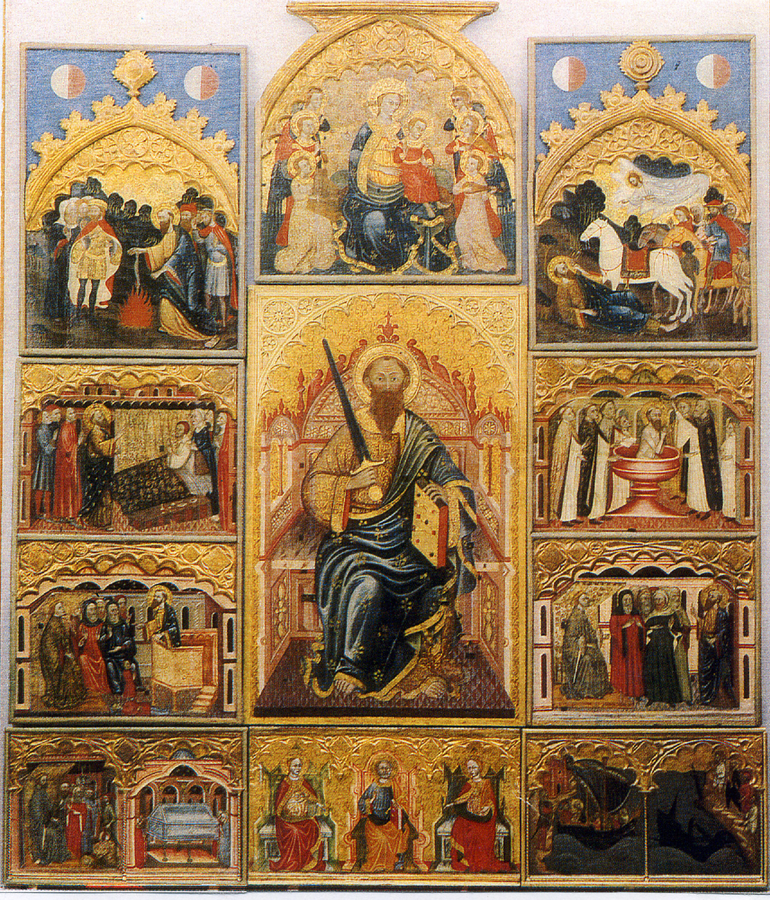
\includegraphics[width=15cm]{pics/front.png}
\end{center}
%\end{comment}
\newpage
\begin{abstract}
The retable is made up of a central panel of St.~Paul Enthroned
surrounded by ten smaller painted scenes, eight of which illustrate
the main events of his life, from his conversion to his death.  The
panels are painted in differing styles, and analysis shows that all
stem from sources traceable to northern Italy, and dated between the
last third of the fourteenth century and the beginning of the
fifteenth.  The same applies to the two upper subsidiary panels that
were later overpainted.  Figure styles, backgrounds, and differing
painting techniques are identified with various concurrent trends:
Veneto-Byzantine, Lombard, and north-European--the latter reflecting
Franco-Flemish work emanating from the great northern centres of
patronage.  In particular, abstract patterns seen on clothing,
furnishings, flooring and backgrounds, are traced individually to
named artists. These artists form part of a total of twelve--for
convenience they are designated the 'Veneto Group'--all belonging to
the generation following that of Guariento di Arpo (documented
1338--1370), and each relating to a particular aspect of the retable.
The St.~Paul retable was thus a collaborative work, and typical of the
current `international' milieu.  In addition, the later overpainting
of certain scenes provides valuable insights into developments in
northern Italy in the painting of figures and of their setting within
a realistic landscape, during what was an important formative period.
\end{abstract}

\vfil

Copyright \copyright\ Joanna Lace 2000, 2010

The moral right of the author has been asserted.

The printed version of this publication, with additional
illustrations, is held by the main libraries in Malta, the Bodleian
Library, Oxford, and the National Art Library, Victoria and Albert
Museum, London.

\subsection*{Acknowledgements}

I would like to express my special thanks to Professor John Cremona of
the University of Warwick for preparing this article for online
publication, and to Mr.~Peter Bartolo Parnis of Malta for the improved
photographs of the polyptic.

\subsection*{Picture credits}

All illustrations of the St.~Paul polyptic are used by the kind
permission of the copyright holder, the Cathedral Museum, Mdina,
Malta, who, whilst allowing access for personal study, wish to
emphasise that no image may be copied or transferred in any manner
without the prior written consent of the Director, any infringement of
this rule being illegal.  

Grateful acknowledgement is also made to the following for permission
to use illustrations as numbered:

Gabriele Corbo: 11; Florence, Centro Di, private collection: 18, 19;
Fratelli Fabri: 12, 14, 15; London, British Museum, British Museum
Press: 45; London, Victoria \& Albert Museum/V \& A Images: 31;
St\"ampfli: 34, 35, 36; Christopher Stylianou: 4.  Washington D.C.,
Dumbarton Oaks Research Library and Collection, Trustees for Harvard
University: 1.

The remaining illustrations are the author's own.  They and short
extracts from the text may be downloaded and printed in an unaltered
form with the prior consent of the author ({\tt
JoannaLace7@gmail.com}), and with the source of the data
acknowledged.

%\begin{comment}

\newpage
\tableofcontents
\section{ Introduction}

This great retable gives an immediate impression of brilliance and
splendour, and its eleven constituent panels have an overall coherence
and harmony conferred by a common palette--deep bright colours
against finely-worked gold--that unifies them chromatically. The
effect is powerful enough to obscure the fact that stylistically they
contain certain interesting divergences, which this paper will
explore.  A detailed analysis reveals that Italian features
predominate, also that these all have their origins in northern Italy
during a period of about forty years from 1367 to c.1407. The
Franco-Flemish and other `oltrealpe' elements to be seen in most
panels date from c.1400 to c.1410, and reflect influences current in
the same region within this same time span.


It is of course to be understood that the evidence does not
necessarily indicate that an Italian provenance is more likely than
one in some outlying region of the Venetian \textit{oltremare}--or
indeed, in any centre of activity in habitual contact with Italian
culture.  The question of a specific provenance for the retable lies
beyond the scope of this enquiry, and will probably have to remain
open until literary evidence comes to light. The same proviso applies
to the question of dating: the commissioning and /or execution of the
panels could have occurred many years after the appearance of Italian
prototypes.

Lack of literary evidence has always led in the past to uncertainties
and differences in attribution\footnote{Past attributions are usefully
summarised in M.~Buhagiar and S.~Fiorini, \textit{Mdina, The Cathedral
City of Malta}, Malta 1996, Part I, p.157. They include: Italy c.1400
(P.~Pullicino 1871); Siculo-Catalan, early 15$^{th}$ century
(V.~Bonello, S.~Botari 1953); Catalonia, circle of Luis Borrassá, c.1410
(G.~Bautier Bresc 1976 and M.~Buhagiar 1987 and 1996).}, as is so
often the case when the main stylistic sources, as here, belong to the
period of the so-called `international style'. For a short period, and
particularly around the year l400, this style was truly
international. This was because artists travelled, often on a
free-lance basis; patronage widened to include wealthy collectors, and
export (especially from Italy) was booming. An affinity developed
between art of widely dispersed regions.  Provenance and dating,
however, can be established in several different ways. When literary
evidence is lacking, and scientific examination not altogether
practicable, then it is that the identification of the artistic
sources that have been used by the artist (or team of artists in the
case of a composite work like the retable) becomes of major
importance. It is therefore with the identification of sources,
iconographic and more particularly stylistic, that this investigation
is concerned.  It is a technique that, as will be seen, resolves some
of the immediate uncertainties.

\section{Preliminary Notes}

\subsection{\textit{Dating}}

No documents have as yet come to light concerning the commissioning or
execution of the retable\footnote{For notes on the primary and
secondary sources for medieval Malta, and a full discussion of the
problems of research, see A.~T.~Luttrell, `Approaches to Medieval Malta'
in A.~T.~Luttrell (ed.), \textit{Medieval Malta: Studies on Malta Before
the Knights}, The British School at Rome, London, 1975, p.1ff, and
ibid., `Girolamo Manduca and Gian Francesco Abela: Tradition and
Invention in Maltese Historiography', in \textit{Melita Historica},
vii, no.2 (1977). An important source for Malta's ecclesiastical
history are the \textit{Acts} of Pietro Dusina's Apostolic Visitation
of 1575; see A.~T.~Luttrell, `Approaches', loc.cit.~above, p.8 and n.53.
}, but a detailed stylistic analysis now accords well with a report
that around 1419 the cathedral was extended eastwards by the addition
of transepts and a short choir\footnote{The main source for the
cathedral building is G.-F.~Abela, \textit{Della Descrittione di Malta
Isola nel Mare Siciliano}, Malta, 1647, pp.331--333; quoted by
M.~Buhagiar, `Medieval Churches in Malta', in A.~T.~Luttrell (ed.),
\textit{Medieval Malta}, op.cit.above, p.178. Abela includes among the
furnishings of the cathedral ``a fifteenth century retable of
St.~Paul''. The cathedral archives record, on 10$^{th}$ January 1477,
the commissioning of Petru di Messina to renew and paint the
``\textit{cortina de lu altaru}'' [the cortina was a painted hanging
installed in front of an altarpiece for protection]; and on 23$^{rd}$
December of the same year the payment to him ``\textit{per la opera de
lu scannellu [predella]}''; and in 1481 the town council authorised
him to receive payment ``\textit{de la cona}'' out of funds belonging
to the Church of St.~Mark. It is considered that had the painting
belonged to that church, its payment would not have involved the town
council, who at that time took an active interest in the
administration of the cathedral; see G.~Wettinger, `Artistic Patronage
in Malta, 1418--1538', in A.~T.~Luttrell (ed.), \textit{Hal Millieri: a
Maltese Casale, its Churches and Paintings}, Malta, 1976, p.111--112
and notes. There is a reference to a bell at the cathedral in a text
of 1645: made in Venice in 1370, and bearing an image of St.~Paul; see
A.~Mifsud, \textit{La Diocesi}, ii (1917/18), p.76--77, quoted in
A.~T.~Luttrell, `Approaches', loc.cit.~above p.20, n.124.}. Such an
event might well have occasioned the commissioning of a major
altarpiece, in keeping with the importance of the site. The date of
its execution, however, remains problematic. During this period
decades could elapse between the commissioning and execution of a
major work. There is ample evidence of this from Sicily, Malta's
dominant neighbour, where patrons were prone to demand richness and
splendour rather than novelty of style\footnote{For contemporary
Sicily, see G.~Bautier Bresc, \textit{Artistes, Patriciens et
Confreries: Production et Consommation de l'oeuvre d'art \`a Palerme et
en Sicile Occidentale (1348--1460)}, \'Ecole Fran\c{c}aise de Rome, 1979.}.

\subsection{\textit{Framing and Assembly}}

As assembled at present, the retable presents the format of the
traditional historiated icon that had evolved from Byzantine art: a
sacred figure surrounded by some of the traditional `stories' of
his/her life. Dismantling and re-assembly, if not outright damage,
doubtless accounts for the lack of vertical buttresses which would
originally have masked lengths of doweling by which main and
subsidiary panels were normally joined together\footnote{For an
account of the development of the historiated icon up to the
fourteenth century, and the diffusion of the ready-made formulae that
artists were trained to use, see Nancy P.~Sevcenko, \textit{The Life of
St.~Nicholas in Byzantine Art}, Turin, 1981.}. For some such reason,
the order of the narrative of the Life of St.~Paul has also notably
been disturbed.  Traditionally, `Lives' begin chronologically with
birth or conversion (in this case, The Road to Damascus), and/or
baptism, followed by preaching/disputing, miracles, and death scenes
last. Accordingly, the `story' panels here flank St.~Paul, running
vertically from top to bottom in two columns, four each side. Clearly,
left and right columns have been transposed at some stage, the
original arrangement being as follows:

\hbox{
{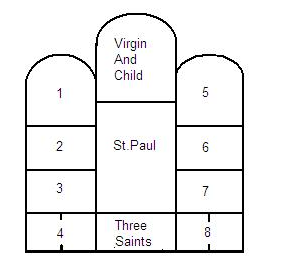
\includegraphics[width=8cm]{pics/plan.png}}
\vbox{
\begin{enumerate}
\item Road to Damascus 
\item Baptism 
\item Disputing 
\item Sea Voyage (combining Departure\\ for Rome and Shipwreck) 
\item Miracle of the Viper 
\item Healing 
\item Raising 
\item Beheading and Veneration
\end{enumerate}
\vskip20pt
}}

The scenes will be referred to in the above abbreviated form in the text.

The wood used--poplar\footnote{Oral communication from Mr.~Samuel
Bugeja, who carried out the most recent restoration work on the
retable.}--was that preferred to all others in northern Italy, and the
subsidiary panels-- roughly square, with rounded tops and finely
cusped-- reflect north Italian work. Also, two distinct methods of
construction have been employed. For the three upper panels and two of
the predella panels, the original carpentry, the application of gesso,
and the background gilding, were all completed before the painting was
begun, and the subsequent painting or repainting of a scene was made
to fit the prescribed area--between cusps, for example. This is the
so-called `Giottesque' or `Trecento' method. The four lateral panels
and one predella panel (the Beheading and Veneration) had frames added
after the painting of the scene had been completed. Studies of Tuscan
and Venetian methods have shown that the Trecento method was not
normally used beyond the first decades of the fifteenth century, and
that during that period both methods existed\footnote{For a useful
study of the stages of altarpiece assembly, and new sequences of
collaboration between \textit{intagliatore} and painter between 1400
and 1450, see C.~Gardner von Teuffel, `The buttressed altarpiece: a
forgotten aspect of Tuscan fourteenth century altarpiece design', in
\textit{Jahrbuch der Berliner Museen}, 21, 1979, pp.21-65.}. It is a
period in keeping both with the style of the finely-worked frames and
with the reported date we gave above for the extension of the
cathedral (1419).

At this point it should be noted that there are features linking the
framing to Spanish work of the time. The first concerns a detail of
the arched frames of the lateral and predella panels: the spandrels
are decorated with a diamond-shaped motif that is found in Aragonese
and Valencian frames\footnote{For example, Pedro Serra
(act.1357-1406), the Retable of San Juan and Santa Luc\'{i}a, in the
Convent of Santo Sepulcro, Zaragoza; Luis Borrassá, the Retable of the
Archangel Gabriel (end of the fourteenth century) in Barcelona
cathedral; illustrated in J.~Gudiol Ricart, \textit{Arte de Espa\~{n}a},
Barcelona, 1955, figs.108 and 280 respectively.}. Also, the vertical
format was one very common in Spain for a large retable, though by no
means confined to that region. However, it will be shown that a
stylistic analysis of the painted scenes points unmistakably to
Italian prototypes. Any specifically Spanish element would in fact
appear to be confined to the \textit{intagliatore}. Clearly there are
unknowns here, and beyond any wishes the patron may have expressed lay
the intricacies of the international market prevailing at the time.

\subsection{\textit{Literary sources of the narrative scenes}}

\begin{enumerate}
\item \textit{The Road to Damascus}

N.T., Acts 9.3-7.  "He saw a light from Heaven, fell to the ground and
heard a voice saying: `Saul, Saul, why do you persecute me?'"

This is sometimes referred to as The Conversion of St.~Paul (or Saul).
The scene has been extensively researched by Thomas Martone, in
\textit{The Theme of the Conversion of Paul in Italian Paintings from
the Early Christian Period to the High Renaissance} (Ph.D.~Thesis),
New York University, 1977.  The author cites all the other New
Testament references to the event, and mentions that the horse came
into the literature with St.~Augustine.

\item\textit{The Baptism}
N.T., Acts, 9.18.

\item\textit{St.~Paul disputing with Festus}: N.T., Acts 25; 

or \textit{St.~Paul disputing with Felix}: N.T., Acts 24.

\item\textit{The Sea Voyage}
N.T., Acts 27.2 and 27.44. 

\item\textit{The Miracle of the Viper}
N.T., Acts 28. 3-5.

\item\textit{St.~Paul heals the father of Publius}
N.T., Acts  28.8.

\item\textit{The Raising of Eutychus at Troas}
N.T., Acts 20. 9-12, 
or  \textit{The Raising of Patroclus in Rome}

Acts of Paul, X, The Martyrdom, paragraphs I and II
(trans.~M.~R.~James, \textit{The Apocryphal New Testament}, Oxford
1953, pp 293-4).

The precise occasion is problematic: the New Testament story of
Eutychus certainly describes a night scene ``with many lamps'', as in
the retable scene, but it could also refer to the Patroclus story
because a woman is present (behind the curtain on the left): she would
be Candida, wife of the chief prison governor, who ``listened and
believed'' and converted her husband.  Also, Patroclus, Nero's
cup-bearer was, like Eutychus, described as a ``lad''. The Troas
story, on the other hand, would not require the presence of an
imperial ruler, but this may be a reference to contemporary dramatic
performances (see Section II below and note 20).

\item\textit{The Beheading of St.~Paul} and
\textit{The Veneration at the tomb of St.~Paul }
Acts of Paul, as cited above, paragraphs V and VII (op.cit.~above, pp
295 and 296).     

In this account Paul said to Longus and Festus (the prefect and the
centurion) ``Come quickly to my grave in the morning, and ye shall
find two men praying, Titus and Luke''.

\end{enumerate}

\subsection{\textit{Points of Iconography}}

\subsubsection*{\textit{The Road to Damascus}}

A horse appeared in this scene in Germany and in Italy during the
twelfth century.  Most relevant to the Mdina version, where the horse
is standing and faces left, is the one in the Giustiniani New
Testament, fol.~128v, in the Giustiniani Collection in Venice, which
has been dated stylistically to c.1200, and is said to be
Veronese.(Fig.1)
\begin{figure}[htbp]
\centering
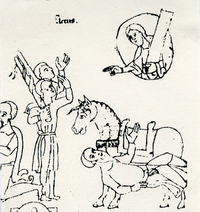
\includegraphics[width=5cm]{pics/fig1.png}
\caption[Veronese School: The Conversion of Paul]
{\it Veronese School: The Conversion of Paul, from the
  Giustiniani Codex, fol.~128v., c.~1200(?).  Venice, Giustiniani
  Collection.} 
\end{figure}


Where Paul is shown falling violently, as in some other versions, the
source is probably the Golden Legend, which specifically states that
Paul was ``thrown''.

\subsubsection*{\textit{The Baptism}}

Baptism was almost exclusively used to illustrate conversion.  The use
of a baptism `shell' or other receptacle (rather than the placing of a
hand) is west European. In the Mdina version the older ritual of
immersion has been combined with that of the aspersion (sprinkling)
method: the latter practice seems to have taken over completely in
France in the fourteenth century, in Italy in the fifteenth, and in
England in the sixteenth. Fonts in medieval Europe (where infant
baptism had become the norm) changed from ancient sunken models to the
raised type of the Mdina scene. Ananias appears as an elderly man in
ecclesiastical garments from the twelfth century in Italy (for
instance, in the mosaic cycles of the Capella Palatina and of
Monreale, in Sicily).

\subsubsection*{\textit{The Sea Voyage}}

A Roman official oversees the departure from Sidon. The voyage
proceeds from left to right (the usual iconography), the wind filling
the sails as it takes the boat seawards.  The captain, also following
tradition, is shown in the stern, controlling a variety of ropes; Paul
is seated beside him. The Giustiniani codex mentioned above is among
the few surviving medieval cycles of St.~Paul that include the
shipwreck.


\subsubsection*{\textit{The Healing of the Father of Publius}}

Some healing scenes show a cure performed by a grasping or active
pulling up of the sick person (including some Veronese manuscripts and
a Neapolitan Bible now in Vienna), but the Mdina version is more
common in Western Europe.  In this, the healer approaches from the
left with a gesture of blessing, the sick person sits upright, hands
joined in prayer (sometimes, as here, attended by members of the
household).

\subsubsection*{\textit{The Raising}}

The duplicate narrative (the boy depicted twice, both dead and raised,
in the same scene) was a medieval device that continued well into the
fifteenth century.

\subsubsection*{\textit{The Beheading}}

In the Acts of Paul, when Paul was beheaded, milk spurted ``upon the
soldier's cloak''; this feature may have appeared originally in the
Mdina scene, or the artist misread his model and depicted blood. The
Acts of Paul, like the Golden Legend (with its account of the three
fountains) omits a feature very common in art, that is taken from the
apocalyptic Passion of Peter (a text attributed to St.~Linus, Peter's
successor as Pope).  This is the veil that Paul borrows from
Plautilla, to bind his eyes before he is beheaded--also absent from
the Mdina scene. The beheading often takes place out-of-doors (in
Sienese works, for example)--with or without Plautilla's veil; and
fountains appeared in Roman versions (Old St.~Peter's, and its
derivative at San Piero a Grado, near Pisa). The executioner is shown
in the Mdina version sheathing his sword, with Paul's head lying
severed on the ground. This is the iconography widely used in Italy;
in other cases, including Spanish examples, an executioner is shown in
the act of raising his arm and about to swipe his victim with his
sword.

\subsubsection*{\textit{The Veneration}\rm
\ \ (Addendum, added March 2010):}

%This is a simple lying-in-state, or vigil.  In Byzantine art, as in
%some versions by Paolo Veneziano (?--1362), the sarcophagus remains
%open.
%
This rectilinear sarcophagus or arca, with steeply inclined gable lid,
free-standing on six columns, is a significant example of the type set
up for the relics of Dominic Guzman, founder of the Order of
Preachers, in the church of San Domenico in Bologna.  This was
completed in 1267 to Nicola Pisano's design, and was soon afterwards
imitated all over Italy, particularly for the tombs of saints and
beati, and particularly among the Dominicans: just as their preaching
was conceived to appeal to the common worshipper, a free-standing arca
enabled devotees to touch it, to benefit from the properties of the
relics within.  See A.F. Moskowitz, \textit{Nicola Pisano's Arca di
  San Domenico and Its Legacy}, Pennsylvania State University Press,
1994.
%

\subsubsection*{\textit{ The Predella Saints: St.~Agatha, St.~Peter,
  St.~Catherine of Alexandria}}

The \textit{spoglie} of St.~Agatha are in Verona cathedral. Until the
sixteenth century they were housed in a \textit{tempietto} outside the
walls, between the Porta Nuova and Porta San Zeno.  (For further
details see C.~Benagha, \textit{La SS. Trinita `in Monte Oliveto' di
Verona}, Verona, 1974; also, with details of Veronese patronage in the
fourteenth century, see (ed.) Giorgio Borelli, \textit{Chiese e
monasteri a Verona}, Verona, 1980.)  In the Mdina predella she is
shown with her usual emblems: her severed breasts on a plate, and the
palm of martyrdom (c.f.~many examples in Sicily, where she holds a
cross). The fact that she is crowned in the Mdina version may be due
to the artist's use of the same \textit{cartone} as for St.~Catherine
of Alexandria, whom the literature refers to as of noble birth, and is
usually crowned. There are notional links between St.~Agatha and
St.~Peter (who, by appearing to St.~Agatha in a vision, cured her
wounds); also between St.~Catherine of Alexandria, the successful
advocate and philosopher, and St.~Peter, whose gesture is that of a
teacher. St.~Peter, again, had from ancient times been seen with
St.~Paul. However, St.~Agatha has always been revered in Malta, and
the choice of saints may have been made by the patron of the retable
for quite other reasons.

\subsubsection*{\textit{The Virgin and Child}}

The unusual feature of this panel is its placing on the upper
(subsidiary) register--the position that is often taken by an
Annunciation or a Piet\`a (Venice), or a Crucifixion (Tuscany).  It is a
point that may be explained only when facts are known as to how the
retable came to be commissioned, and by whom. An altarpiece in
Sardinia (mentioned below, note 24) also has a Virgin and Child with
Two Donors in the main pinnacle. Other points of the iconography of
this panel (the lack of veil, the musicians) are covered below
(Section IV).

\section{ Stylistic Analysis}

\subsection{\textit{St.~Paul Enthroned}}

Taking as starting point the large central panel, three aspects point
towards the Veneto: the head, the modelling technique, and the throne
(Fig.2).
\begin{figure}[htbp]
\centering
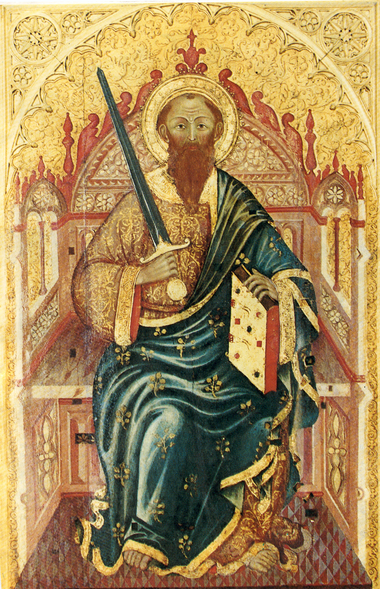
\includegraphics[width=10cm]{pics/fig2.png}
\caption[The Mdina retable of St.~Paul, centre panel, St.~Paul
  Enthroned.]
{\it The Mdina retable of St.~Paul, centre panel, St.~Paul Enthroned.
The Cathedral Museum, Mdina, Malta. \copyright\ The Cathedral Museum,
  Mdina, Malta.} 
\end{figure}
Most arresting is certainly the head, whose stylised facial
features belong to a time-honoured tradition for a devotional image
(using proportions arrived at by means of a modular system).  They
produce that aesthetic and somewhat severe cast of face familiar in
all icons and other works of art having their common source in
Byzantium.  In the present context, however, their byzantine linearity
has been set within a naturalistic bone-structure--characteristically
wide at the temples -that is particularly associated with hierarchical
figures of the fourteenth century Sienese school\footnote{For example,
in Simone Martini's great \textit{Maest\`a} of 1315 in the Palazzo
Publico, Siena (see \textit{L'Opera Completa di Simone Martini},
Classici dell'Arte, Milan, l97O, Tav.~l); Lippo Memmi's
\textit{Maest\`a} in the Palazzo del Podesta, San Gimignano, of 1317
(see L.~Bellosi (Introd.), \textit{La Pittura dell'Italia centrale
nell'et\`a gotica}, I Maestri del Colore, 252, Milan, l966, Tav.~20);
A.~Lorenzetti's \textit{St.~Peter} and \textit{St.~Paul}, in the
Church of St.~Peter and St.~Paul, Roccalbegna, of c.~1320 or c.~1340
(see E.~Borsook, \textit{Ambrogio Lorenzetti}, Florence, 1966,
Figs.~76 and 77); Giacomo di Mino del Pellicciaio, \textit{Head of
St.~Anthony} of l362, in the Pinacoteca, Siena (see M.~Meiss,
\textit{Painting in Florence and Siena after the Black Death},
Princeton, USA, 1979, Fig.~61).}.  Particularly close to the Mdina
head in this respect is the head of St.~Paul in a panel, now in Paris,
from an altarpiece by an artist of the second generation of this
school, dated between c.~1350 and c.~1375\footnote{See M.~Laclotte
(ed.), \textit{Retables Italiens du XIIIe au XVe si\'{e}cle}, Les dossiers
du d\'{e}partement des peintures, 16, Paris, 1978, No.~10:
\textit{St.~Paul} (from the Church of Saint-Louis-en-l'\^{I}le, Paris).
It has been variously attributed to Luca di Tomm\`e, Bartolo di Fredi,
and Lippo Vanni (see loc.~cit., pp.~21-22).}. (Fig.3) 
\begin{figure}[htbp]
\centering
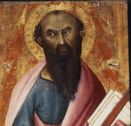
\includegraphics[width=4cm]{pics/fig3.png}
\caption[Sienese School: St.~Paul, c.1360-65]
{\it Sienese School: St.~Paul, c.1360-65.  Paris, Church of
Saint-Louis-en-l'\^Ile.}
\end{figure}
This is not to
say that the Mdina artist necessarily had any connection with Siena,
because by this period styles from Sienese workshops had not only been
taken up throughout Italy, but had spread abroad with the movement of
artists between the various courts of Europe.  A Sienese element is no
indication of location--either of prototype or copy--but it does
indicate influence, and therefore provides a useful \textit{terminus a
quo}.  The close combination of `ancient' and `modern' (i.e.~byzantine
and Sienese) clearly demonstrates the continuing preference (either of
artist or of patron) for an ancient hieratic formula, during a period
when artists were rapidly developing more naturalistic forms for other
sections of a composite work.

In this connection it is notable that the Mdina artist has also kept
to an ancient byzantine tradition for the Saint's ears: they are
abnormally large, and turned forward ``to receive the word of
God''. They have a particular morphological feature, the Y-shaped
motif within the shell of the ear, that was also widespread during the
fourteenth century. Artists of the Veneto were amongst those
occasionally using this motif\footnote{These include Simone dei
Crocefissi (documented 1355--c.1399), for example his panel Pope
Urban V of c.1370, now in the National Gallery, Bologna (see
catalogue, Bologna 1987, no.44 p.29); and in works attributed to
Niccol\`o di Pietro (documented 1394--1430), for example the lateral
wings of a polyptych of St.~Francis and St.~Louis of Toulouse, now in
the Mus\'ee du Petit Palais, Avignon (see M.~Boskovits, \textit{The
Martello Collection}, Florence 1985, p.124).}.

From a stylistic point of view, the technique used in this panel for
the drapery of St.~Paul's mantle is more revealing.  The heavy
modelling by means of stereotyped white motifs is the work of an
artist trained in a well-attested byzantine technique. The broad knee
patch (a characteristic ovoid swirl) and sweeping prong-like shapes
for the shoulder folds, constitute a simple code for distinguishing
convex from flat surfaces--a method that had become widespread
throughout Eastern Europe by the early fourteenth century
(e.g. Cyprus, Fig.4),
\begin{figure}[htbp]
\centering
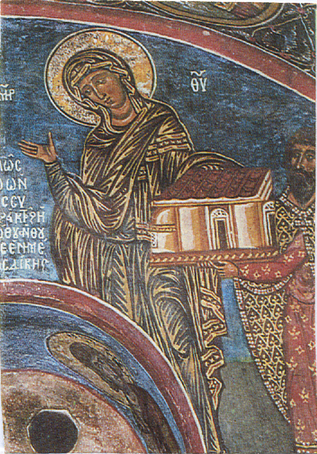
\includegraphics[width=7cm]{pics/fig4.png}
\caption[Fresco of The Donor Presenting the Church to Christ
  through the Virgin (detail)]
{\it Fresco of The Donor Presenting the Church to Christ
  through the Virgin (detail), c.1350--c.1375.  Asinou, Cyprus,
  Church of the Panagia Phorbiotissa.}
\end{figure}
and continued in use in the Veneto, the region
of Italy with close ties with the East\footnote{Amongst examples of
the style, in Trieste: fresco of the Death of the Virgin, end of the
14$^{th}$ century, now in Museo Civico, Trieste; in Serbia: frescoes
in the Monastery of Gra\u{c}anica, Kosovo, of 1321 (illustrated in
O. Bihalji-Merin, \textit{Byzantine Frescoes and Icons in Yugoslavia},
London, 1960, e.g. Plate 57: The Raising of Lazarus); and frescoes
signed and dated by Micajlo and Eutichije in the Church of St.~George,
Staro Nagori\u{c}ino, of 1317-18 (illustrated in O. Bihalji-Merin,
op. cit., e.g. Plate 52: The Mocking of Christ (detail, standing
figure in foreground)). For examples in Cyprus: the mid-14$^{th}$
century fresco of the Nativity in the Church of St.~Nicholas of the
Roof, Kakopetria (south arm of the nave), illustrated in A. \&
J.~A.~Stylianou, \textit{The Painted Churches of Cyprus}, London, 1985,
Fig. 28; fresco of the Ascension of Christ, of the third quarter of
the 14$^{th}$ century (after 1353) in the Church of the Holy Cross,
Pelendri (north side of the east vault), illustrated in A. \&
J.~A.~Stylianou, op. cit., Fig. 129); and fresco of the Donor
presenting the church to Christ through the Virgin, of the same
period, in the Church of Panagia Phorbiotissa of Asinou, central nave,
illuminated in A.~\&~J.~A.~Stylianou, op.cit., Fig.57. Amongst many
examples from the furthermost regions of influence, is a late
fourteenth century Novgorod icon of The Descent into Limbo, now in the
Russian Museum, St.~Petersburg; illustrated in D. Likhachov et al.,
\textit{Novgorod Icons 12th--17th Century}, Oxford-Leningrad, 1980,
Plate 58. For the addition, in byzantine painting in general, of
broader patches of light colour for modelling, as introduced in the
13$^{th}$ century and refined by the Paleologue painters of the early
14$^{th}$ century, see John Stuart, \textit{Ikons}, London, l975,
chap. 4.}.

It was the Italian Veneto that produced the specific combination seen
in the Mdina St.~Paul Enthroned, where byzantine modelling accompanies
flat passages emulating rich brocade. Two particular features of
St.~Paul's brocade are also relevant here.  It has been simulated by
the application of gold to a preliminary ground colour (the Venetian
method\footnote{In Tuscany, on the other hand, artists perfected the
\textit{sgraffiato} technique, where the ground, rather than the
motif, is gold. For the development of these techniques, and more
sophisticated examples by Sienese artists, see Simone Martini's
\textit{Maest\`a} of 1315 and works of Pietro Lorenzetti of the 1320s,
illustrated in Paul Hills, \textit{The Light of Early Italian
Painting}, Yale University, 1987, Chapter VI, Fig. 60 and Colour Plate
XXII.}); and the way the regular pattern of gold arabesques packs the
prescribed area closely, and without foreshortening, points to a stage
in decorative patterning stylistically near to the early work of Paolo
Veneziano (?--1362) and his workshop, and quite consistent with
versions by the less experimental of his many followers. It is notable
also that a particular version of decorative `Kufic' lettering used by
Paolo is identical to that on the golden cuffs of St.~Paul
Enthroned\footnote{See Paolo Veneziano, with sons Luca and Giovanni:
The Finding of the Body of St.~Mark, 1345. Venice, panel of the
covering of the Pala d'Oro, Museo Marciano.}.

St.~Paul's throne accords well with these findings: it is a
single-arched adaptation of the throne in the great fresco of the
Coronation of the Virgin by Guariento di Arpo (documented 1338 -
1370), that decorated the end wall of the Sala del Maggior Consiglio
in the Ducal Palace in Venice from 1365/7--1577 (when it was damaged
by fire\footnote{It is often referred to simply as the
`\textit{Paradiso'}, and its full title is: The Coronation of the
Virgin and the Court in Heaven; see J. White, \textit{Art and
Architecture in Italy: 1250-1400}, Pelican History of Art,
Harmondsworth, 1987, illus. 350 (detail); also F.~F.~D'Arcais,
\textit{Guariento, Tutta la Pittura}, Venice, 1974, Figs. 121-127.
For the documentation, see F.~F.~D'Arcais, op. cit., pp. 72-73.}).
Guariento, a well-established Paduan artist, had been called to Venice
to decorate this sala. His ultimate source for the throne lay fifty
years earlier in the pinnacled structure that Simone Martini and his
brother-in-law Lippo Memmi had created for the \textit{Maest\`a} for the
Palazzo Publico at Siena (1315)\footnote{See \textit{L'Opera Completa
di Simone Martini}, op. cit. above (note 9), loc. cit. It was copied
by Memmi in his \textit{Maest\`a} for the Palazzo del Podesta at San
Gimignano, in 1317; see \textit{La Pittura dell'Italia Centrale
nell'et\`a Gotica}, op.cit. above (note 9), Tav.20.}. Guariento
introduced unprecedented spatial depth, by using strongly defined
orthogonals, and by showing the shafts of the side arcading in
recession--all features repeated here.  The vast composition proved
to be his masterpiece, and the throne in particular was much
imitated\footnote{Derivatives include those in works by Jacobello del
Fiore (1370-1439): his Coronation of the Virgin of l438, commissioned
by the Bishop of Ceneda (Vittorio Veneto) and now in the Galleria
dell'Accademia, Venice (see Ildiko Ember, \textit{Music in Painting},
Budapest, 1984, No. 9); and Giovanni D'Alemagna and Antonio Vivarini:
Coronation of the Virgin, signed and dated 1444, in the Church of San
Pantalon, Venice (see G. Lorenzetti, \textit{Venice and its Lagoon},
Rome, 1961, illus. p. 572). Jacobello and artists of his workshop have
recently been brought together under the name of the `Master of
Ceneda'; they belong to the group I have designated in Part II as the
`Veneto group'. Jacobello is also amongst members of this group who
may have worked with Gentile da Fabriano on the second stage of
decoration of the Sala del Maggior Consilio during the early years of
the 14$^{th}$ century (see below note 81).}. By 1367 Guariento had
returned to Padua, so we have a \textit{terminus post quem} for the
Mdina derivative.

\subsection{\textit{The Four Lateral Scenes}}

The four lateral scenes (the Baptism, Disputing, Healing and Raising)
are all interiors, and their common architectural setting marks them
off as a group (Figs. 5,6,7 and 8). 
\begin{figure}[htbp]
\centering
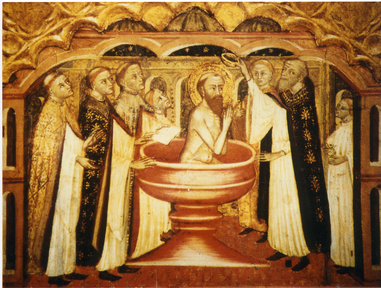
\includegraphics[width=10cm]{pics/fig5.png}
\caption[The Mdina retable of St.~Paul, lateral panel, The Baptism
  of St.~Paul]
{\it The Mdina retable of St.~Paul, lateral panel, The Baptism
  of St.~Paul. 
The Cathedral Museum, Mdina, Malta. \copyright\ The Cathedral Museum,
  Mdina, Malta.} 
\end{figure}
\begin{figure}[htbp]
\centering
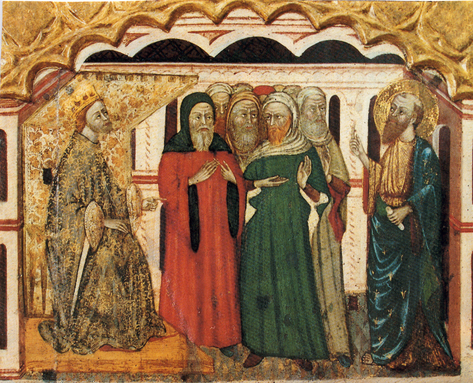
\includegraphics[width=10cm]{pics/fig6.png}
\caption[The Mdina retable of St.~Paul, lateral panel, St.~Paul
  Disputing]
{\it The Mdina retable of St.~Paul, lateral panel, St.~Paul Disputing.
The Cathedral Museum, Mdina, Malta. \copyright\ The Cathedral Museum,
  Mdina, Malta.} 
\end{figure}
\begin{figure}[htbp]
\centering
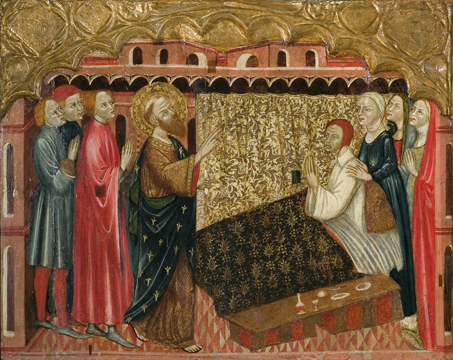
\includegraphics[width=14cm]{pics/fig7.png}
\caption[The Mdina retable of St.~Paul, lateral panel, The Healing of the
Father of Publius]
{\it The Mdina retable of St.~Paul, lateral panel, The Healing of the
Father of Publius.  
The Cathedral Museum, Mdina, Malta. \copyright\ The Cathedral Museum,
  Mdina, Malta.} 
\end{figure}
\begin{figure}[htbp]
\centering
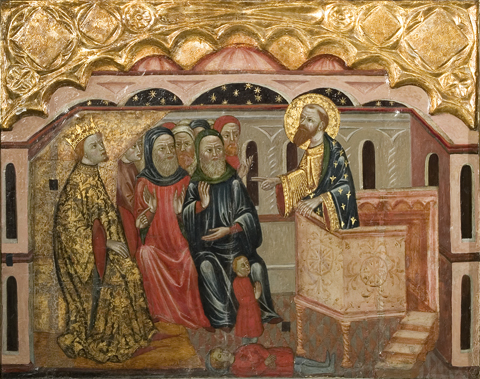
\includegraphics[width=14cm]{pics/fig8.png}
\caption[The Mdina retable of St.~Paul, lateral panel, The Raising
  of Eutychus, or of Patroclus]
{\it The Mdina retable of St.~Paul, lateral panel, The Raising
  of Eutychus, or of Patroclus.  
he Cathedral Museum, Mdina, Malta. \copyright\ The Cathedral Museum,
  Mdina, Malta.} 
\end{figure}
I shall first analyse this somewhat complex background.  I shall then
consider aspects of figural style and items of furniture, relating
these features to the main panel.

The layout of all four scenes is identical, pointing to the repeated
use of the same \textit{cartone}, and this was a favourite Paduan
method for producing narrative, found in frescoes of the 1360s and
1370s. It was used by Guariento in his St.~Philip cycle (c. 1368) in
the Church of the Eremitani\footnote{See C.~L.~Ragghianti,
\textit{Pittura tra Giotto e Pisanello: Trecento e Primo
Quattrocento}, Civilt\`a artistica a Ferrara, 2, Ferrara, 1987,
illus. 14, St.~Philip Ordered to Sacrifice to the Idol, and The
Miracle of the Cross. The date is disputed: on stylistic grounds some
scholars consider this fresco cycle to come before the Venice
\textit{Paradiso} of 1367/8; others, including Ragghianti, consider it
to be post-1368.}, and in the mid-1370s Giusto de' Menabuoi
(documented 1363--87), a highly successful newcomer to Padua from
Florence, used it in his decorative programme, the \textit{Stories of
Esau}, in the drum of the baptistery of Padua cathedral\footnote{See
C.~L.~Ragghianti, op. cit. above (note 18), illus. 19.  Giusto's own
origins lay in Florence, but he is documented as living in Padua by
1370, and his most important works, of the 1370s, are there. See also,
M. Gregori, `La Presenza di Giusto a Viboldone', in \textit{Paragone},
293, 1971, pp. 3 ff. and Tav. 21. Gregori refers to a more complex
theory that Giusto's \textit{persistenza ambientale} stemmed from the
late antique method of narration used in the mosaics of the Genesis
cycle of the early 13$^{th}$ century in St.~Mark's, Venice--a cycle
said, in its turn, to reflect an ancient byzantine prototype, the
Cotton Genesis.}.  It has been explained, not as a means of economy of
work, but as presenting a \textit{persistenza ambietale} that
developed out of medieval drama, where successive scenes would be
shown, sometimes with minor modifications, against the same
background, even when distances of time and place were being
presented\footnote{Regarding dramatic performances, it is interesting
that the Dominicans (prominent protagonists in the Mdina Baptism
scene) were the first to stage mystery plays--in Milan--from 1366;
see E. M\^ale, \textit{L'Art R\'{e}ligieuse de la fin du Moyen Age en
France}, Paris, 1922, p. 69 ff.  See also C. Molinari, `Spectacoli
Fiorentini del Quattrocento', in \textit{Racolta Pisana}, 5, Venice,
1961, p. 128.}.

It is not implied by this that a Paduan artist produced the
\textit{cartone} for the background matrix.  The latter has one
feature, in fact--the blind arcading for the walls of these interiors
- that is too widely dispersed in art by the second half of the
fourteenth century to be any guide as to provenance. The same could be
said in general regarding the insertions above these walls of the
external roofs of buildings. In respect of the domes however, in the
Baptism and Raising panels, these are a particular hallmark of church
architecture in Venice and in Padua, and studies by H. Buchtal on
Sicilian illumination have suggested that artists were prone to take
models and give them a local \textit{ambiente} (by the addition, in
the case of Palermo, of Mohammedan-type domes)\footnote{See H.~Buchtal,
`Early Fourteenth-Century Illuminations from Palermo' in
\textit{Dumbarton Oaks Papers}, 20 (1966), p.108-109.}. The Mdina
matrix may well have been modified for the same reason. A fresco in
Ferrara of the first decades of the fifteenth century certainly has
similar domes placed in this way. Again, the flat-roofed arcaded
building in the Healing panel has its closest parallel in a
\textit{frontale} of the same period painted in Padua, depicting the
Legend of S. Giovanni Boccadoro. (Fig.9)
\begin{figure}[htbp]
\centering
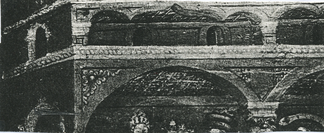
\includegraphics[width=8cm]{pics/fig9.png}
\caption[The Compagno Ferrarese (attrib.): The Legend of
  S. Giovanni Boccadoro (detail)]
{\it The Compagno Ferrarese (attrib.): The Legend of
  S. Giovanni Boccadoro (detail), c. 1420-40.  Modena, Galleria Estense.} 
\end{figure}
Both fresco and panel
painting have recently been attributed by C.~L.~Ragghianti to an artist
active in Padua during the first decades of the fifteenth century,
whom he refers to as the `Compagno Ferrarese'\footnote{The fresco, The
Presentation of Christ in the Temple, from the Church of S. Guglielmo,
Ferrara, and now in the Casa Romei, Ferrara, was previously attributed
to the GZ Master (a Veronese or Paduan artist in the circle of
Altichiero), and to the circle of the Ferrarese artist Antonio
Alberti. The Ferrarese \textit{frontale}, the Legend of S. Giovanni
Boccadoro, is now in the Galleria Estense, Modena. Both fresco and
panel painting are illustrated in C.~L.~Ragghianti, op. cit. above (note
18), illus.78 and illus. 210 respectively.}. To sum up, these
architectural additions are a first indication that, just as the
repetitive use of a matrix for a narrative cycle was common in Padua,
the interiors themselves may have been produced by an artist or
artists working in the same milieu. It is when the rest of the
background architecture is fully examined that a number of other
stylistic features imposed upon the matrix are all found to be part of
the Paduan repertoire of the followers of Guariento of the succeeding
generation.

During the fourteenth century two particularly influential artists
evolved systems by which architectural forms were used to indicate the
interior of a building.  One was Giotto (?1267--1337), particularly
active in Padua and in Naples, and the other was Ambrogio Lorinzetti
(active 1319--1347).  The Mdina matrix is a combination of both
systems.  Solutions to the problem of creating three-dimensional
interior space were often a combination of several prototypes, which
were imperfectly understood.

The Giottesque element in the lateral panels consists in the way all
four interiors are framed each side by narrow sections of exterior
wall (complete with paired openings) shown in elevation: this is an
abbreviated reference to Giottesque solutions in which the exterior of
a building was always shown.  Precisely the same design is seen in
Angevin Naples, in work of the 1330s and 1340s attributed to
`Giottesque' artists: for example, the sculptured scenes of the Story
of St.~Catherine of Alexandria from Santa Chiara\footnote{Attributed to
Giovanni and Pacio da Firenze, documented 1343-45; see J. White,
op. cit. above (note 15), p. 451 and Fig. 277.}, and again in a panel
depicting the Birth of St.~Nicholas of Bari, in the predella of an
altarpiece in Sardinia by the `Maestro delle Tempere
Francescane'\footnote{In the cathedral of Ottana, Sardinia, dated
c. 1340; see F. Bologna,\textit{ I Pittori alla Corte Angioina di
Napoli,1266-1414}, Rome, 1969, Tav. VI--26, 32.  Bologna refers to
the spread of ``the Giottesque culture of the Maestro delle Tempere
Francescane'' to Sicily, Aragon, and Avignon, around this date.}. By
the late 1350s it had appeared in italianate frescoes at the Imperial
Court of Bohemia\footnote{For example in the Chapel of the Virgin in
Karlstein Castle, Prague, dated 1357 (right hand of east wall).
Prague was the emergent artistic and cultural centre of Bohemia, and
owed much to artists trained in Italy by the Emperor Charles IV.}. In
the case of the Mdina matrix, these narrow forward sections are
therefore evidence of the carrying over of an old-established system
into a later context, by an artist whose true interest perhaps lay in
balanced rectilinear pattern-making.

The second architectural element is the distinctive so-called
`diaphragm' arch\footnote{I have adopted the term introduced by
E. Panofsky: see his \textit{Renaissance and Renascences in Western
Art}, New York, 1972, p. 142 and note 2; for the way the arch cuts
down the spectator's field of vision and hides the point where the
orthogonals would touch the margins, see his \textit{Early
Netherlandish Painting}, New York, 1971, Vol. One, \textit{Text},
pp. 58-59.}. Ambrogio Lorenzetti introduced this into panel painting
in a highly sophisticated form in 1342, in his Presentation in the
Temple, (Fig.10)
\begin{figure}[htbp]
\centering
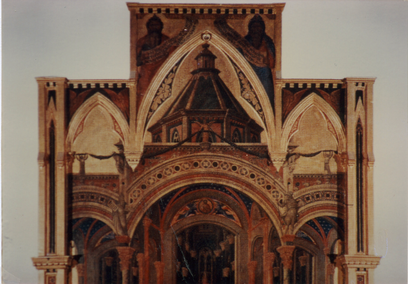
\includegraphics[width=10cm]{pics/fig10.png}
\caption[Ambrogio Lorenzetti: Presentation in the Temple (detail)]
{\it Ambrogio Lorenzetti: Presentation in the Temple (detail), 1342.
Florence, Uffizi Gallery.} 
\end{figure}
and by 1405-8 it had been taken up by the artist
(probably Flemish) known as the `Boucicaut Master', in the Hours of
the Mar\'echal de Boucicaut\footnote{The Ambrogio Lorenzetti work is the
centre panel of a triptych, now in the Uffizi Gallery, Florence; see
E. Panofsky, \textit{Renaissance and Renascences}, op. cit. above
(note 26), Fig. 101.  For the Boucicaut Hours, now in Paris, Mus\'ee
Jacquemart-Andr\'e (MS.2), see E. Panofsky, \textit{Early Netherlandish
Painting}, op. cit. above (note 26), Vol. Two, \textit{Plates},
Fig. 62: Vigils of the Dead (fol. 142v.). Panofsky discusses their
style and approximate dating in op.cit. Vol.~One, \textit{Text}, p.53
ff., and refers to the Boucicaut Master's possible stay in Milan,
loc.cit.p.58, note 1. A different use of a diaphragm, where it frames
the view into the interior of a free-standing building, occurs in a
panel of The Flagellation and Other Scenes, of the school of the
Marches, dated to the mid-14$^{th}$ century. It is now in the Museum
of Fine Arts, Valletta, Malta; see D.~Cutajar (ed.), \textit{Museum of
Fine Arts, Valletta}, Malta, 1991, illus.p.7.}. It is a device to lend
spatial depth to a composition: an arch painted in as if overlapped by
the wood frame of the panel, thus coming between the frame and the
picture space. In the Mdina panels this `diaphragm' component
varies. In the ecclestical scenes of the Baptism and the Raising it
stands out clearly: for the Baptism a pinkish brown, contrasting with
the brownish grey of the three church domes appearing above it; and
the colour scheme is reversed for the Raising scene. (Figs.5 and 8) It
duly cuts across the upper part of these two panels, but then instead
of disappearing behind the wood frame to left and right (in order to
increase the visual depth of the scene `beyond'), it is made to merge
with the orthogonals of the side walls, and thus becomes of one piece
with the painted building, thereby negating its original
function. Whatever form any previous wood frames may have had, it is
unlikely that they ever masked completely the ambiguity of these upper
corners.

The diaphragm arches of the secular interiors, the Disputing and
Healing scenes, on the other hand, have been modified so that they do
bridge the picture space independently of the lateral strips of
`outside' wall.  The Disputing has been given a slightly deeper-cusped
diaphragm, and its striated surface completely fills the remaining
upper section of the panel. (Fig.6) In thus including neither `sky',
exterior roofs, nor gold ground, it becomes the kind of `procenium'
favoured by Giusto de' Menabuoi in the 1370s, for example, in his
frescoes with \textit{persistenza ambientale} in the baptistery of
Padua cathedral\footnote{See C.~L.~Ragghianti, op. cit. above (note
18), illus. 19.}. (Fig.11) 
\begin{figure}[htbp]
\centering
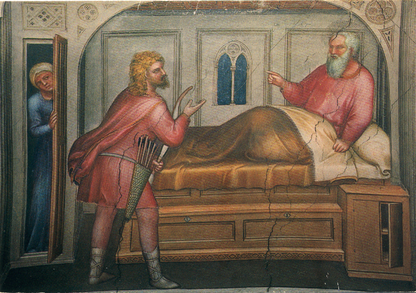
\includegraphics[width=8cm]{pics/fig11.png}
\caption[Giusto de' Menabuoi: Stories of Esau, mid-1370s]
{\it Giusto de' Menabuoi: Stories of Esau, mid-1370s.  Padua, Duomo
(Baptistery).} 
\end{figure}
The Healing (its rear wall almost totally
taken up by a decorative curtain for Publius' father's bedchamber) has
been modified to a still different design: a smaller-cusped diaphragm,
cutting across the panel horizontally to clear the taller figures, the
space above it showing the flat roofs of the secular building
(Publius' palace?) against a gold ground. (Fig.7) In both these
modified scenes the artist certainly shows each end of the diaphragm
disappearing beneath the wooden frame, and neatly masking the corner
orthogonal intersections of the painted architecture, in true
Lorenzettian fashion.

The form of the matrix itself is thus of mixed parentage, and has
suffered from a flux of evolving theories.  These theories were
circulating widely not only in Italy, but equally in Burgundy and
Bohemia during the latter part of the fourteenth century.  The Mdina
version however, has been given certain decorative details that were
used by artists who worked in the Veneto during the 1360's and 1370's.
First, the use of deep or pinkish red for coping and dado edges in all
four scenes, nicely stressing three-dimensionality: this had appeared
early in the century in Padua, in Giotto's influential decorative
scheme in the Arena Chapel, completed about 1313\footnote{See
\textit{L'Opera Completa di Giotto}, Classici dell'Arte Rizzoli, nuova
serie, Milan, 1978: Presentation at the Temple and Cleansing of the
Temple, Tav. XX and Tav. XXX respectively.}. Guariento's follower,
Nicoletto Semitecolo (active ?1335--1381)--an artist whose name will
be mentioned several times in this survey--used the pink coping in
panels of the \textit{Life of St.~Sebastian}, painted for Padua
cathedral and dated 1367\footnote{See \textit{Paolo Veneziano e il Suo
Tempo}, I Maestri del Colore, No. 241, Tav. X, The Burial of
St.~Sebastian by Santa Lucina and her Companions. The panels are in
the Biblioteca Capitolare in Padua.} (for example Fig.12).
\begin{figure}[htbp]
\centering
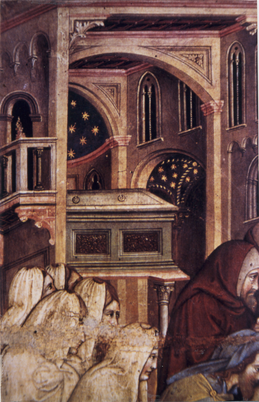
\includegraphics[width=5cm]{pics/fig12.png}
\caption[Nicoletto Semitecolo: The Burial of St.~Sebastian (detail),
  1367]
{\it Nicoletto Semitecolo: The Burial of St.~Sebastian (detail), 1367.
Padua, Biblioteca Capitolare.} 
\end{figure}
Secondly,
the starlit sky glimpsed through the cusped arches of the diaphragm
arch in the Baptism and Raising scenes (but here illogically placed
below the domes) is found in work of both Guariento and Semitecolo
(also in his St.~Sebastian panels)\footnote{For Guariento, see his
(attributed) fresco of The Coronation of the Virgin, formerly
decorating the tomb of Jacopino da Carrara in the Church of
St.~Augustine, Padua, dated c.1351, and now in the Church of the
Eremitani, Padua; illustrated in F.~F.~D'Arcais, \textit{Guariento},
op. cit. above (note 15), Tav. 32.  For Semitecolo, see his panel
depicting The Burial of St.~Sebastian, cited above (note 30).}. In
addition, the unusual dull greyish-brown for walls in these two scenes
(in lieu of the pale pinks and ochres of Lorenzetti followers) is a
particular characteristic of Giusto's painted architecture, for
example in his cathedral baptistery frescos referred to above. The
box-like interiors of the Mdina scenes have a high view-point,
resulting from the way the side walls are made to recede sharply
upwards.  This perspective seems retardaire for the 1370s: at the same
time it is an occasional feature of the paintings of Stefano Veneziano
(\textit{plebanus,} di Sant'Agnese, active c.1369--1384), an artist
who was working with Semitecolo in Venice 1380--1381. The backgrounds
of these lateral scenes in fact show stylistic devices that are not
always fully understood, but they are all, nevertheless, consistent
with the sources identified in the main panel of St.~Paul Enthroned,
and with its post-1368 dating.

The same can be said of another decorative detail that has appeared at
some stage in the Disputing and Healing scenes, and that creates
further spatial ambiguity.  This concerns the diaper pattern, in black
upon a brown ground, and which has also been inserted differently into
each scene. In the Disputing it is placed above a horizontal rear wall
(decorated with small cusping) and below the procenium-type arch. It
thus fills the space which the modern eye reads as `sky'. (Fig.6) In
the Healing the diaper is placed not above, but below a horizontal
diaphragm with small cusping. The patterning thus tends to be read as
`wall-paper', filling the narrow space above the brocade
curtain. (Fig.7) These intrusions into complex background architecture
that is Italian in origin, suggest the intervention of an artist,
quite possibly a non-Italian, more used to the older and simpler
convention of filling backgrounds (both external and interior spaces)
with abstract pattern\footnote{On the use of background patterns, see
M.~S.~Bunim, \textit{Space in Medieval Painting and the Forerunners of
Perspective}, New York, 1940.}. But they do not rule out the Veneto as
provenance, because foreign artists often worked side by side with
Italians: for instance under the patronage of the ardent francophile
Giangaleazzo Visconti of Milan (1351--1402), who already by the 1380s
ruled Verona and Padua. Furthermore, a series of illuminated
manuscripts of the \textit{Tacuinum Sanitatis in Medicina}, datable to
c. 1380--1400 and from this region, includes examples of the
self-same black-on-brown diaper design as the Mdina scenes
(e.g. Fig.13). 
\begin{figure}[htbp]
\centering
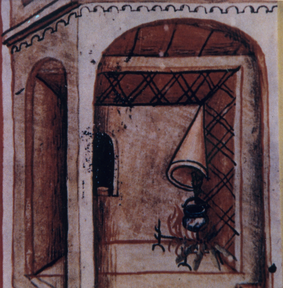
\includegraphics[width=5cm]{pics/fig13.png}
\caption[Workshop of Giovannino de' Grassi (attrib.): Aqua Calida
  (detail)]
{\it Workshop of Giovannino de' Grassi (attrib.): Aqua Calida (detail),
from the \textit{Tacuinum Sanitatis in Medicina}, c. 1380-c. 1400.
Vienna, \"Osterreichische Nationalbibliothek, Codex Vindobonensis,
Series Nova, 2644, fol. 89.} 
\end{figure}
The series will be discussed later in reference to
similarities in figural style and technique, all of which make more
likely some connection between the Mdina panels and a Visconti
workshop\footnote{See below note 55.}.

It is clear from the foregoing that the backgrounds of these lateral
scenes point to artists conversant with works of the Veneto of the
last decades of the fourteenth century or the first years of the
fifteenth, and an analysis of the figure styles will show that they
also are consistent with these sources and with their dating. They are
not, however, related--like the matrix--to the work of Guariento or
his followers, and differ in two important respects: in their
disposition, which still derives ultimately from long-established
medieval formulae for narrative, and in individual features of build,
stance, and physiognomy. The latter owe nothing to the new dynamism of
Guariento's compositions, nor to his heavier neo-Gothic figure style.

To begin with the general disposition of the figures: the Mdina work
follows a tradition in which the creation of a pleasing pattern was
the prevailing interest, and, given the exigencies of the chosen
iconography, this was achieved by means of the balanced arrangement of
the figures, largely uncluttered, and set close to the picture
plane. The demand for narrative clarity was met by placing the main
protagonist(s) either centrally (as in the Baptism), or setting them
slightly apart from the rest (in the Disputing, Healing, and Raising),
and by massing any subsidiary figures into closely packed, often
isocephalus, groups.  Action was limited to the gestures of hands, the
positioning of feet, and direction of gaze, all of which usually gave,
as here, an impression of arrested movement, and a certain tenseness
of expression.  That this remained the accepted narrative form in
Venice for some important commissions in various media, is shown by
the miniatures of a Venetian \textit{istoria} of c.1340-70 considered
by scholars to reflect an important fresco cycle within the Ducal
Palace complex\footnote{The manuscript, in Venetian dialect, is the
\textit{Libro della Leggenda degli Apostoli Pietro e Paolo, di
S. Albano e della venuta a Venezia di Papa Alexandro III}, Venice,
Biblioteca del Museo Correr, Cod. Correr I, no. 383 (=1497); see
P. Fortini Brown, \textit{Venetian Narrative Painting in the Age of
Carpaccio}, Yale University, 1989, Plates V--VIII. Its date is
disputed; Fortini Brown (op. cit., p. 260) favours a date near to
1370.  The frescoes, in the Church of San Nicol\`o, were completed by
1329, and were still in place in 1400 (later destroyed); for full
documentation see P. Fortini Brown, op. cit., pp. 37-38, notes 17 and
18, and Catalogue II.}, and by the mosaics added to the Basilica of
San Marco at around the mid-century\footnote{Illustrated in
S. Bettini, \textit{Mosaici di San Marco}, Milan, 1968, pp. 44 and 45
(Chapel of St.~Isidore), and p. 46 (baptistery).}. (Fig.14)
\begin{figure}[htbp]
\centering
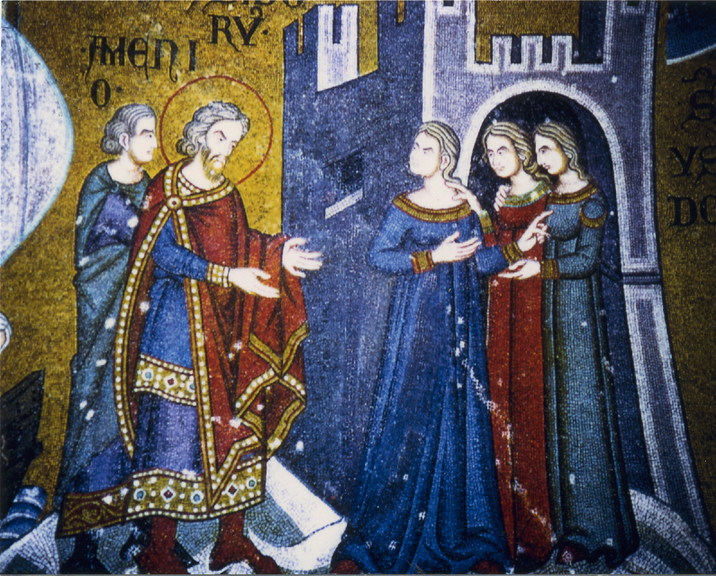
\includegraphics[width=10cm]{pics/fig14.png}
\caption[Venetian School: St.~Isidore Preaching, mosaic of 1342-54]
{\it Venetian School: St.~Isidore Preaching, mosaic of 1342-54.
Venice, San Marco, Cappella di Sant'Isidoro.} 
\end{figure}

Regarding the figures in these subsidiary panels individually, no
single gratuitous swirl or sway of drapery been brought in anywhere
for dramatic emphasis. Displaying no concern with any such artifice,
garments are made to fall in simple vertical folds, in accordance with
a continuing, older-established tradition. In the Baptism and Healing
panels this calm, dignified style is associated not only with
monumental works in Venice itself, such as the miniatures and mosaics
already cited, but with a range of fresco cycles of the second half of
the fourteenth century by Lombard artists that has survived in
provincial centres of the Veneto, Emilia, and Lombardy.  These cycles,
like the Mdina panels, include elongated figures with a specifically
northern feature: this is the characteristic `northern' or `Lombard'
head, having rounded contours, a sharp, often retrouss\'e nose, a high
forehead, and often red `bobbed' hair. It was a style common to the
whole of northern Italy (not limited to the boundaries of modern
Lombardy) and Bohemia\footnote{Amongst numerous examples in northern
Italy, see those illustrated in \textit{Gli Affreschi Gotici
Lombardi}, Part 2, I Maestri del Colore, No. 225, Milan, 1966.  For
Bohemia, see (ed.) E. Bachmann, \textit{Gothic Art in Bohemia},
London, 1977: for example, Plate VI, Jan Ocko von Vl\={a}\v{s}\'{i}m votive
panel of c. 1371-1375, now in the National Gallery, Prague. It is
notable that when Prague became the Imperial capital, the Emperor
Charles IV (d. 1377) brought in mosaicists from the Veneto to
embellish new buildings. Semitecolo, for example, is thought to have
supplied the \textit{cartone} for the mosaic of Christ the Judge
placed on the south transept facade of the Cathedral of St.~Vitus: the
figure of St.~Vitus has a typical `boyish' northern head. See
R. Pallucchini, \textit{La Pittura Veneziana del Trecento},
Venice-Rome, 1964, Fig. 710.  The influx of Italian styles into
east-central Europe generally, is extensively covered in M. Prokopp,
\textit{Italian Trecento Influence on Murals in East Central Europe,
particularly Hungary}, Budapest, 1983.}. (Fig.15) 
\begin{figure}[htbp]
\centering
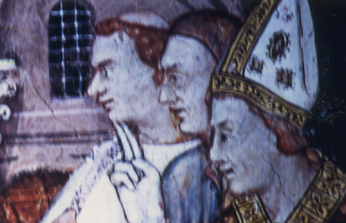
\includegraphics[width=8cm]{pics/fig15.png}
\caption[Lombard School: Translation of the Body of St.~Stephen,
  1375-80]
{\it Lombard School: Translation of the Body of St.~Stephen (detail), 1375-80.
Lentate, Oratorio di Santo Stefano.} 
\end{figure}
The head of St.~Paul
in each panel, on the other hand, has the gaunt, pinched physiognomy
associated with the Veneto-byzantine idiom that was adhered to by
followers of Paolo Veneziano. The most renowned of these was Lorenzo
Veneziano (active 1356? -- 1372)\footnote{Early examples include the
main central panel of the Santa Chiara Triptych, attributed to the
Master of the Santa Chiara Triptych, and sometimes linked with
contemporary Venetian miniatures (see M. Boskovits, \textit{The
Martello Collection}, op.cit. above note 11, pp 90-93). The triptych
comes from the church of the Poor Clares of Santa Maria della Cella,
Trieste, and is now in the Museo Civico, Trieste; see exhibition
catalogue \textit{Pittura su tavola dalle collezioni dei Civici Musei
di Storia ed Arte di Trieste}, Trieste 1975, section II.1.}. (Fig.16)
\begin{figure}[htbp]
\centering
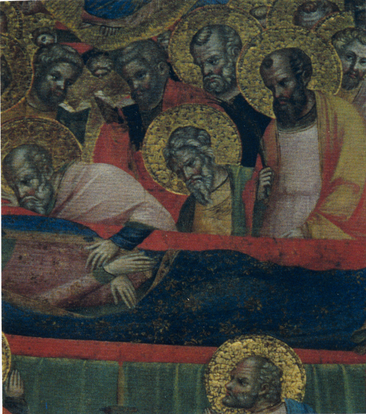
\includegraphics[width=8cm]{pics/fig16.png}
\caption[Lorenzo Veneziano: The Death of the Virgin (detail)
  1366]
{\it Lorenzo Veneziano: The Death of the Virgin (detail)
  1366. Vincenza, cathedral, Proti chapel.}  
\end{figure}
Otherwise the traditional Lombard head appears throughout the retable
for female figures and for the unbearded males, giving the latter the
typically `boyish' appearance seen in many of the frescoes mentioned
above.

In the Disputing and Raising scenes, heavy beards are combined with a
different broad physiognomy (Fig.17). 
\begin{figure}[htbp]
\centering
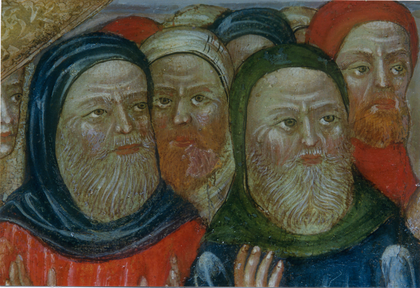
\includegraphics[width=8cm]{pics/fig17.png}
\caption[The Mdina retable of St.~Paul, lateral panel, The Raising
  of Eutychus or of Patroclus (detail)]
{\it The Mdina retable of St.~Paul, lateral panel, The Raising
  of Eutychus or of Patroclus (detail).  
The Cathedral Museum, Mdina, Malta. \copyright\ The Cathedral Museum,
  Mdina, Malta.} 
\end{figure}
These heads bear the
unmistakable stamp of the new Franco-Flemish naturalistic style that
appeared in Italy, in various media, towards the end of the century.
They show a striking likeness, in fact, to robust heads by Andr\'e
Beauneveu (1330 -- 1403/13, working for Jean, Duc de Berry) and by
Claus Sluter (c. 1350 -- 1406), whose work at the Burgundian court at
Dijon was widely influential in disseminating this new
trend\footnote{In this paper I shall use the term `Franco-Flemish' to
include artists from Flanders who spent periods in Paris, and so came
under the influence of French styles. For Sluter, see for example the
figures of his Well of Moses, executed for Philip the Bold, Duke of
Burgundy, at the Chartreuse de Champmol, near Dijon, dated 1395-1400
(now in the grounds of the Psychiatric Hospital, Dijon, with replica
in the Mus\'ee des Beaux-Arts, Dijon); see E.~H.~Gombrich, \textit{The
Story of Art}, London, 1950, Fig. 152: The Prophets Daniel and
Isaiah. For Beauneveu, see The Psalter of Jean de Berry, c.1386 (24
grisailles): e.g. fol.19, The Prophet Joel, illustrated in M.~Thomas,
\textit{The Golden Age, Manuscript Painting at the Time of Jean, Duke
of Berry}, New York, 1979, Plate 12; also see sculptures of prophets
dated 1392--1405 attributed to his circle (now in the Municipal
Museum, Bourges); illustrated in exhibition catalogue \textit{Les
Fastes du Gothique, le si\`ecle de Charles V}, Paris, 1981,
Cat. 224. The new style was introduced into Tuscan monumental
sculpture by Lorenzo Ghiberti (1378 or 1381 to 1455), for his figures
on the north doors of the baptistery of Florence cathedral; he won the
competition for this commission in 1401; the doors are recorded as
almost finished in 1417.  See K. Clark and G. Robinson, \textit{The
Florence Baptistery Doors}, London, 1980, Fig. 149, Panel XIX, The
Entry into Jerusalem. Ghiberti's use of this style reflects either
close contact with French artists at the Angevin court in Naples, or
else direct knowledge of northern developments.}. The Veneto need not
be excluded as a source: miniatures of certain specifically Venetian
manuscripts dated from c.1385 show the same technique of long loose
brush strokes for beards that similarly cover half the
cheek\footnote{See M. Boskovits, \textit{The Martello Collection},
op.cit. above (note 11) Cat. 43, p. 147: illuminated leaf with the
Ascension of Christ and Two Prophets.}. (Fig.18) 
\begin{figure}[htbp]
\centering
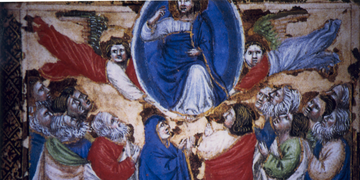
\includegraphics[width=10cm]{pics/fig18.png}
\caption[Venetian School: The Ascension of Christ and Two
  Prophets, a page from a Book of Hours (detail)]
{\it Venetian School: The Ascension of Christ and Two
  Prophets, a page from a Book of Hours (detail), last quarter of the
  fourteenth century. Florence, Private collection.}
\end{figure}
Also, amongst
contemporary panel painters of Venice and the Veneto whose broad
Flemish facial types carry the heavy characterisation of the Mdina
`elders', two named artists are particularly relevant.  They are
Zanino di Pietro Veneziano (active 1389--c. 1406), and a Veronese
artist, Giovanni Badile (1379--1451), connected with Zanino's circle
early in his career. The precise identity of Zanino is unclear. The
catalogue of his reported activities is typical of many artists of
this `international' period. It encapsulates, in fact, most of the
artistic influences that will be identified within the retable: he was
possibly French; he is said to have had contacts with Flemish artists,
including the influential Melchior Broederlam (court painter from 1385
to Philip the Bold, Duke of Burgundy, in Dijon); he probably spent a
long period in Bologna before his arrival in Venice in 1405; in Venice
he designed tapestries for St.~Mark's for execution by Franco-Flemish
workers, and executed his only signed work, a triptych of the
Crucifixion, dated 1405\footnote{Now in the Museo Civico, Rieti; see
(ed.) L. Magagnato, \textit{Da Altichiero a Pisanello}, Venice, 1958,
Tav. LVII.  Recent scholarship suggests that Zanino should be
identified with the artist Giovanni di Piero Charlier, or Giovanni di
Francia, documented in Venice between 1404 and 1432, and again with
Zanino Peroni, documented in Bologna between 1389 and 1406.  See
S. Padovani, `Una Nuova Proposta per Zanino di Pietro', in
\textit{Paragone}, nos. 419-421-423, 1985, pp. 73-81; and
M. Boscovits, \textit{The Martello Collection}, op. cit. above (note
11), p. 148.}.  However, closest stylistically to a bearded Mdina
`elder' (especially the red-bearded figure with white hood in the
Disputing and in the Raising scenes) is a head of St.~John the
Evangelist in a panel attributed to the early years of Badile: here,
unmistakably, is the peculiar sharpness of facial features of Mdina,
that produces a characteristic expression of watchful
intensity\footnote{See M. Boscovits, \textit{The Martello Collection},
op. cit. above (note 11), p. 31, St.~John the
Evangelist.}. (c.f. Figs.17 and 19)
\begin{figure}[htbp]
\centering
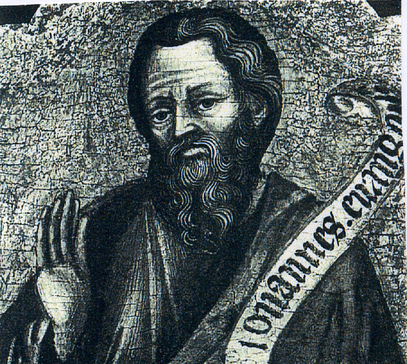
\includegraphics[width=6cm]{pics/fig19.png}
\caption[Giovanni Badile (attrib.): St.~John the Evangelist,
  beginning of the fifteenth century]
{\it Giovanni Badile (attrib.): St.~John the Evangelist (detail),
  beginning of the fifteenth century.  Private collection.}
\end{figure}

So far our investigation has traced the design of both St.~Paul
Enthroned and the architectural backgrounds of the lateral panels to
sources current in the Veneto from the late 1360s onwards. Some types
of physiognomy seen in the panels then suggested a collaboration
between artists trained in several different milieux: the traditional
north Italian (common to Lombardy and Bohemia); the Veneto-byzantine;
and a non-Italian, Franco-Flemish tradition that is datable to
c. 1400. It remains to consider how details of dress, stance, and
finally interesting differences in painting technique, relate to these
conclusions.

In isolation the style of dress for secular figures would be of little
help in a situation where fashions--like art forms--were common to
different European courts, and which, moreover, were not always
perfectly `in step'. The French styles worn by the young companions of
St.~Paul in the Healing scene are a case in point: for one a belted
\textit{supertunica} just covering the knee\footnote{This garment
tended to become shorter as the fourteenth century progressed;
covering the knees, it would indicate, when worn at court, a date not
later than c. 1380. In art, however, the possibility of a later
imitation of a prototype, or of a provincial or \textit{retardaire}
milieu, must equally be borne in mind.}, and, for the other, just
behind St.~Paul, an ankle-length \textit{houppelande}\footnote{A loose
wide-sleeved collarless gown. The version in the Mdina scene, where
the sleeves are left ungathered at the wrist, was worn in court
circles until c. 1410.}. Similar examples in dated French, Bohemian
and Italian manuscripts span at least half a century from around the
1360s, and the bonnet known as a \textit{calette} or \textit{kalle}
worn by Publius' father was popular even longer\footnote{It was worn
by men from the twelfth to the fifteenth century in all Latin
countries, and could occur in the art of neighbouring regions
(e.g. the Balkans), not necessarily from a prototype, but merely to
indicate an elegant (i.e. `French') lifestyle; see A. Grabar, `Un
reflet du monde latin dans une peinture balkanique du 13e si\`ecle', in
\textit{Byzantion}, I, 1924, pp. 229-243.}. Fortunately, in the Mdina
scenes important clues as to dating and source are provided by certain
stylistic details of hands and feet. These include the boat-shaped
feet of the standing figures in the Baptism scene; also a particular
arrangement for a group of walking figures, where the long shoes are
placed in `sloping' parallel rows, as in the Healing scene. (Fig.20)
\begin{figure}[htbp]
\centering
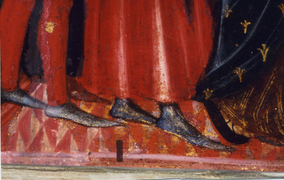
\includegraphics[width=10cm]{pics/fig20.png}
\caption[The Mdina retable of St.~Paul, lateral panel, The Healing of the
Father of Publius (detail)]
{\it The Mdina retable of St.~Paul, lateral panel, The Healing of the
Father of Publius (detail).  
The Cathedral Museum, Mdina, Malta. \copyright\ The Cathedral Museum,
  Mdina, Malta.} 
\end{figure}
They reflect French compositions of the second half of the fourteenth
century\footnote{Amongst many examples are those in the miniatures of
The Coronation Book of Charles V of France (BL. MS. Cotton,
Tib. B.VIII), dated 1365; see (ed.) E.S. Dewick, \textit{The
Coronation Book of Charles V of France}, London, 1899, especially
Col. Plate I, and black/white illus. 1 and 2; also those of the
\textit{Grandes Chroniques de France de Charles V} (Paris Bib. Nat.,
MS.fr.2813) of c.~1375-1379; and the \textit{Pelerinages} by Guillaume
de Digueville (Paris Bib.~Nat., MS.fr.823), dated 1393; see \textit{Les
Fastes du Gothique}, op. cit. above (note 38), Cat. 284 and Cat. 294
respectively.}, but at the same time such stylistic features, as well
as identical details of dress, are attested in miniatures executed in
Verona and Padua during the same period. Examples include those of a
recension of Petrach's \textit{De Viris
Illustribus}\footnote{Darmstadt, Landesbibliothek, MS.101, illustrated
in G.~L.~Mellini, `Disegni di Altichiero e della sua Scuola, 1' in
\textit{Critica d'Arte}, 51, 1962, p.1 ff., Figs 14-27.}, a
\textit{Titus Livius} of c.1373\footnote{Milan, Biblioteca Ambrosiana,
Cod. 214 inf. (Prima Deca); see, for example, R.~Pallucchini,
op.cit. above (note 36) figs. 702--705.}, and others also attributed
to the influential school of Altichiero, the acknowledged successor of
Guariento. The long French shoes \textit{\`a la poulaine}, protruding
from the regal robes in the Disputing and Raising scenes, whilst
reminiscent of French and Franco-Flemish examples, also appear in late
fourteenth century work by Lombard artists, who in particular favoured
such extremes of fashion, even for religious scenes\footnote{For
instance, the late fourteenth century fresco cycle of the Life of
St.~Catherine, attributed to a Lombard artist, from the Church of
S. Lorenzo, Piacenza (Chapel of St.~Catherine), and now in the Museo
Civico, Piacenza; see catalogue, ed. S.~Pronti, \textit{Il Museo Civico
di Piacenza in Palazzo Farnese}, Piacenza, 1988, illus. pp. 120 and
122, and Tav.~VI.} (Fig.21).
\begin{figure}[htbp]
\centering
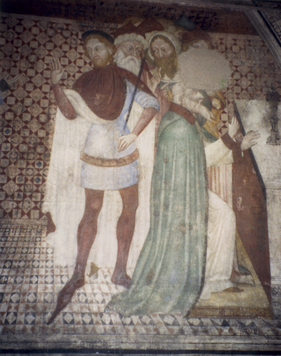
\includegraphics[width=5cm]{pics/fig21.png}
\caption[Lombard School: The Dispute of St.~Catherine with the Philosophers(?)
(detail)] 
{\it Lombard School: The Dispute of St.~Catherine with the Philosophers(?)
(detail), last decades of the fourteenth century.  Piacenza, Museo
Civico.}
\end{figure}
Both the Lombards and their Bohemian
colleagues working in the border regions of the Alto Adige and South
Tyrol, featured the \textit{poulaine} in their lively scenes of
courtly life--scenes that also included other figural details of the
school of Altichiero.  In the Alto Adige, for example, at Trent (a
cycle of \textit{The Months} in the Bishop's apartments in the Torre
Aquila), and at nearby Castelroncolo, there are well-preserved
examples amongst the vast programmes carried out in fresco by these
artists for their wealthier patrons\footnote{The frescoes in Trent
were commissioned by the Bishop, and are dated c. 1400; see
E. Castelnuovo, \textit{Il Ciclo dei Mesi di Torre Aquila a Trento},
Trent, 1987, especially p. 57: Maggio (second floor, south wall).  For
those at Castelroncolo, dated 1388-1395, and c. 1400, see M.~Frei,
\textit{Castelroncolo}, Bolzano, 1984, illus. 3.}. To sum up, then,
the subsidiary figures in these Mdina scenes show features of the
north Italian courtly style of the late fourteenth century.

The same cannot be said of the figure of St.~Paul in these panels,
whose classicizing ecclesiastical garb has not been exchanged for
contemporary courtly dress, as was the case for holy persons from the
1360's in the St.~Sebastian panels by Semitecolo, for example
(Fig.22), 
\begin{figure}[htbp]
\centering
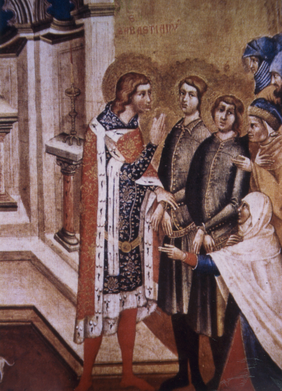
\includegraphics[width=5cm]{pics/fig22.png}
\caption[Nicoletto Semitecolo: St.~Sebastian Encourages Two Christians
(detail)] 
{\it Nicoletto Semitecolo: St.~Sebastian Encourages Two Christians
(detail), 1367.  Padua, Biblioteca Capitolare.}
\end{figure}
and in the sophisticated milieu of Verona\footnote{For
Semitecolo, see Maria Prokopp, \textit{Great Masters of the Trecento},
Budapest, 1986, No.45: Saint Sebastian Encourages Two Christians. A
courtly style for saintly figures had long been part of the Veronese
tradition: a fresco in the Church of S. Zeno, St.~George Frees the
Princess, sometimes attributed to the young Altichiero, is one notable
example. St.~Paul is also shown in `cavalier' dress in miniatures by
the Veronese artist Turone and his workshop: e.g. Corale MXVII and
Corale MXLVIII, in the Biblioteca Capitolare, Verona; see
E. Sandberg-Vaval\`a, `Turone Miniatore', in \textit{Daedalo}, X, 1929,
p. 15ff. Turone's only securely-dated work is an altarpiece of 1360,
and the \textit{corali} are considered to be dated slightly
later.}. However, the ancient traditional iconography--that is to
say, the depicting of all sacred figures as ecclesiastics--was still
current in northern Europe during the second half of the fourteenth
century, and in work of Italian artists influenced by northern
contacts, including much provincial church decoration in northern
Italy. The same applies to a small stylistic detail of St.~Paul's
drapery in the Disputing scene, which remained a northern convention
for painting floor-length garments that in Italy was more commonly
seen in northern regions. This is the fold at ground level which wraps
the protruding foot closely, creating a `tube' or `funnel' motif. It
is part of a long-established repertoire, referring back to Romanesque
models, and more often introduced, as in the Mdina Disputing, for a
full-length figure, when it was deemed necessary to show at least one
foot\footnote{Examples in English illumination occur in the so-called
Douce Apocalypse of c. 1270: Oxford, Bodleian Library, MS.~Douce 180,
p. 66, The Angel with the Fifth Vial of Wrath; see G. Henderson,
\textit{Gothic}, Penguin Books, 1978, Fig. 45.  Mid-14$^{th}$ century
Bohemian examples include the Vyss\'i Brod altarpiece of c. 1350; see
J. Pesina, \textit{Mistr Vysebrodsk\'eho Cyklu}, Prague, 1987, Fig. 35,
The Crucifixion (the figure of St.~John). In the Parisian Angers
Apocalypse tapestries of 1375-1381, examples include a Scene at the
Chateau, Angers; see A. Martindale, \textit{Gothic Art}, London, 1979,
Fig. 173.}. (Fig.23) 
\begin{figure}[htbp]
\centering
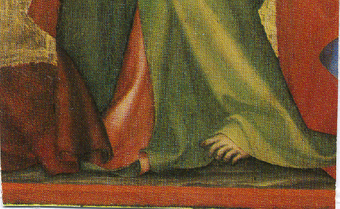
\includegraphics[width=8cm]{pics/fig23.png}
\caption[Bohemian School: St.~Bartholomew and St.~Thomas (detail)] 
{\it Bohemian School: St.~Bartholomew and St.~Thomas (detail), from the
Epitaph of St.~John of Jeren, 1395.  Prague, National Gallery.}
\end{figure}
Not unexpectedly this motif is one of the
northern features seen in a tapestry design for St.~Mark's, Venice,
attributed to Zanino, one of the artists referred to above in
connection with his Franco-Flemish figural types\footnote{See
\textit{Il gotico internazionale} in Italia, I Maestri del Colore,
No. 255, Milan, 1966, Doc. 2: The Incredulity of St.~Thomas. The
tapestry is now in the Museo Marciano, Venice.}.

A final piece of evidence links the figure of St.~Paul in the lateral
panels to the Alto Adige.  This concerns a Bohemian artist, Meister
Wenzeslaus, or `Venclaus', who signed a fresco cycle in the cemetery
chapel adjacent to the Church of Our Lady at Riffiano, near Merano,
dated 1415\footnote{The precise identity of `Venclaus' is disputed;
for references to past discussions see \textit{L'Opera Completa di
Gentile da Fabriano}, Classici dell'Arte, Milan, 1976, p.93, catalogue
nos.59-62, with bibliography and with illustrations of works variously
attributed in the past to Venclaus, Nicolo di Pietro, the young
Pisanello, as well as to Gentile.}.  The cycle, like other provincial
art in the region, has figures with physiognomy close to that of
Mdina.  Meister `Venclaus' is thought by some scholars to be the
artist of the courtly cycle of \textit{The Months} mentioned above in
connection with the \textit{poulaines}; this was commissioned by the
Bishop, George of Lichtenstein, for the Torre Aquila in Trent, and is
dated to c. 1400.  Whether or not this particular theory is entirely
convincing, it is reasonable to suppose that parts of such a vast
programme were the work of a team.  And it is at Trent, amongst the
subsidiary decoration on the second floor of the Torre Aquila, that
attention is drawn to a morphological detail that is also a salient
characteristic of the Mdina figures of St.~Paul: a thin wrist, and,
for the right hand (the `speaking' hand) exceptionally long, curved
`squared-off' fingers\footnote{See E. Castelnuovo, op. cit. above
(note 49): frontispiece (detail of frieze round west
window).}. (Fig.24) 
\begin{figure}[htbp]
\centering
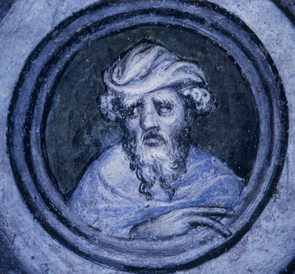
\includegraphics[width=7cm]{pics/fig24.png}
\caption[Unknown artist: wall decoration (detail), c. 1400] 
{\it Unknown artist: wall decoration (detail), c. 1400.  Trent, Torre
Aquila.}
\end{figure}
These small details help to reduce the wide field
introduced by the designation `Lombard' for build, stance and
physiognomy of certain Mdina figures. The evidence now suggests, in
effect, a date near the turn of the century, with current French
fashions set in the context of the border regions of the Alto Adige.

The fact that the courtly element in northern Italy at this time was
Lombard reflects in general terms the supremacy, over other northern
courts, of the court centred on Milan and Pavia under Giangaleazzo
Visconti, powerful patron of the arts (Fig. 25). 
\begin{figure}[htbp]
\centering
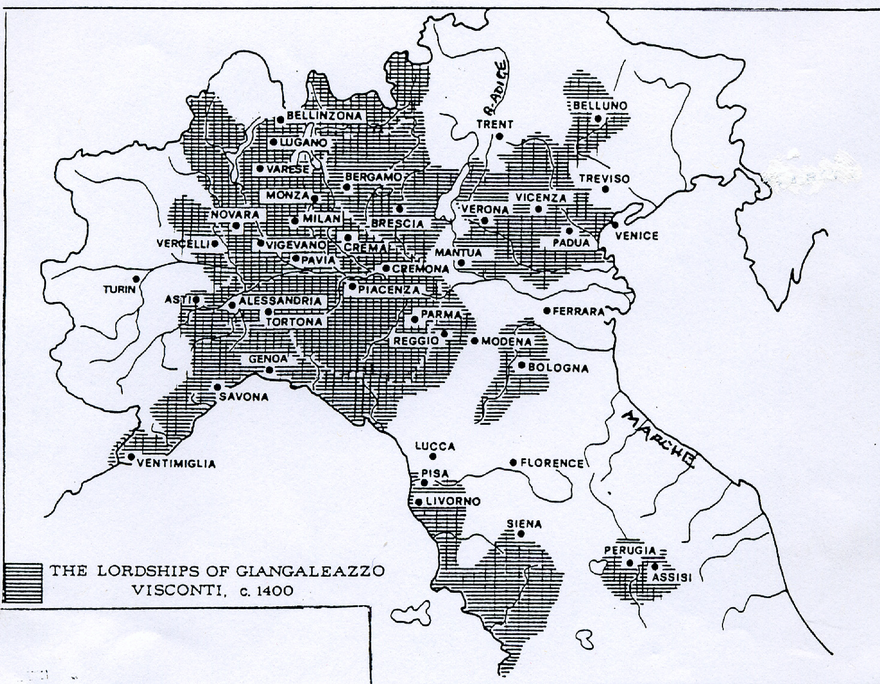
\includegraphics[width=15cm]{pics/fig25.png}
\caption[The Power of the Visconti, c.1400.] 
{\it The Power of the Visconti, c.1400.}
\end{figure}
One group of
illuminated manuscripts, produced in a workshop under his patronage,
not only shows figures with all the general characteristics of
St.~Paul's companions in the Healing scene (Lombard heads with
`bobbed' hair, court dress in blues and reds) but, in the case of the
manuscript now in Vienna, the particular style of the
\textit{poulaines}, which are characteristically reduced to mere wisps
of red colour (e.g. fol.10v, \textit{Nespula,} Fig.26). 
\begin{figure}[htbp]
\centering
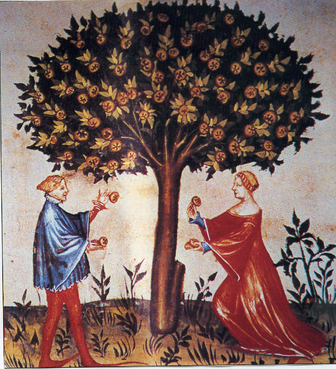
\includegraphics[width=8cm]{pics/fig26.png}
\caption[Workshop of Giovannino de'Grassi (attrib.): Nespula, from the
\textit{Tacuinum Sanitatis in Medicina} c. 1380-c.1400] 
{\it Workshop of Giovannino de'Grassi (attrib.): Nespula, from the
\textit{Tacuinum Sanitatis in Medicina} c. 1380-c.1400.
Vienna, \"Osterreichische Nationalbibliothek, Codex Vindobonensis,
Series Nova, 2644, fol. 10v.}
\end{figure}
The group is a
series of recensions of the \textit{Tacuinum Sanitatis in Medicina},
and was referred to earlier in this section, in that several
miniatures feature the same diaper pattern that has been inserted in
the architectural backgrounds of the Disputing and Healing scenes. The
\textit{Tacuinum Sanitatis} was a reference book of herbal medicine
translated from the Arabic, circulating in the Lombardy and Veronese
regions. All the known illuminated versions were produced in the
aristocratic ambience of either Verona or Pavia between c.1380 and
c.1400\footnote{The rich libraries of Pavia and Verona were
amalgamated after 1387, when Giangaleazzo conquered Verona from the
ruling Scaliger family. For the Vienna manuscript, \"Osterreichische
Nationalbibliothek, Codex Vindobonensis, Series Nova, 2644, see (ed.)
J. Spencer, \textit{The Four Seasons of the House of Cerruti}, New
York and Bicester, England, l988.  The manuscript bears the arms of
Bishop George, and available evidence suggests it was completed before
l403. The various copies are fully discussed in L.~Cogliato Arano,
\textit{The Tacuinum Sanitatus in Medicina}, London, 1976 (also Milan
1979).}. They were illuminated by different artists, their common
source probably being a pen and ink version of c. 1380, only partly
coloured, and bearing the name of Giovannino de' Grassi (c. 1340 -
1398), a pre-eminent miniaturist and architect at Giangaleazzo's
court, and the whole group has recently been ascribed to Giovannino's
workshop.

In the light of the evidence linking Mdina figure styles to this
prestigious workshop as well as to the Alto Adige, it is particularly
interesting to find that precisely the Vienna \textit{Tacuinum},
mentioned above, has been shown to have been acquired around the turn
of the century by the wealthy Bishop of Trent--the same Bishop George
of Lichtenstein, in fact, who during his bishopric (1390--1407)
commissioned the cycle of \textit{The Months} for his newly-converted
apartments in the Torre Aquila. With this manuscript not only in
Trent, but in the possession of a notable patron of the arts, the Alto
Adige becomes a candidate as the source not only for northern
characteristics (which were found to relate to artists such as Badile,
Zanino and Wenzeslaus), but for a well-defined courtly element as
well.

If specifically Venetian features seem less obvious at this point, the
balance begins to be redressed when modelling is taken into account,
and here again the \textit{Tacuinum} miniatures serve as a useful
comparison. In the miniatures, for instance, the modelling technique
is tonal, with changes in tone following the natural shape of objects.
This produces modelling reminiscent of the so-called `soft style' of
Bohemia, a painterly, naturalistic style, adumbrating the delicate
atmospheric effects that became a hallmark of the Lombard school of
illumination.  Patterned objects, as well as those in plain colours,
are discreetly modelled in this way\footnote{Examples in Bishop
George's copy include a table-cloth and a bed cover; see J. Spencer,
op. cit. above (note 55), p. 125 (chapter heading) and p. 133
(`Wakefulness') respectively.}. In the Mdina panels, on the other
hand, for areas in plain colour there are two systems in operation:
the Lombard modelling of the \textit{Tacuinum } is juxtaposed with
sharp Veneto-byzantine motifs on the shoulder and knee areas of the
figures in blue--the Veneto-byzantine technique, in fact, of
St.~Paul's blue robe in the main Mdina panel. The contrast between the
two systems is particularly striking in the Raising scene. (Fig.8) The
patterned areas in the panels, notably the bed-cover in the Healing
scene, and the decorated copes of the prelates in the Baptism, have
large gold motifs on a saturated ground and are not colour-modelled at
all. They thus correspond, in turn, to the system used for St.~Paul's
brocaded tunic in the main panel, that was found to belong to the less
sophisticated decorative system used by Venetian followers of Paolo
Veneziano.

The Veneto-byzantine technique that thus links the four lateral scenes
with the main votive panel of St.~Paul Enthroned is not unexpected. By
the same token, the style and presentation of the furniture in these
four scenes (regal thrones, ambo, and font) are as consistent with a
source in the Veneto, as is the great throne of St.~Paul. Although not
uniquely Venetian, similar types all appear in works executed in the
Veneto during the fourteenth century\footnote{The form of the regal
thrones, and of the ambo, are common to the fourteenth century art of
France and the Veneto. The simple throne occurs in the St.~Ursula
altarpiece by Paolo Veneziano (see R. Pallucchini, \textit{La pittura
veneziana del Trecento}, op.cit. above (note 36), Fig. 42); and the
ambo features in sculptures of the Life of St.~Peter Martyr on the west
facade of the Church of St.~Anastasia, Verona, as well as in
miniatures of a French work, The Coronation Book of Charles V of
France, dated 1365, cited above (note 45), fol.64; illustrated in
J.~White, \textit{The Birth and Rebirth of Pictorial Space}, London,
1972, Plate 51c. The design depicted on the side of the Mdina ambo
appears as a motif in wall decorations of 1354--1376 in the
Castelvecchio, Verona. The Mdina font is a simplified version of the
font in the fresco cycle attributed to Altichiero and other artists in
the Oratory of St.~George, Padua, completed in 1378 (in the scene
where St.~George baptises the King of Cirene, on the south
wall).}. Amongst smaller objects, the carafe on the bedside table in
the Healing scene is, moreover, the classic Venetian type featured as
such in the Glass Museum, Murano, and shown there with examples from
paintings that include again a miniature from the Vienna
\textit{Tacuinum }owned by the Bishop of Trent\footnote{See
J. Spencer, op. cit. above (note 55), p. 63, Vinum album. The carafe
continues to be featured, not only in Italy (for example by
Bartolommeo di Giovanni, active 1485-1510, in A Legend of St.~Andrew,
illustrated in the foreign catalogue of the Walker Art Gallery,
Liverpool, \textit{Plates}, p.10), but in distant regions where
Venetian influence on church decoration persisted: in Cyprus, for
instance, in a fresco depicting the Hospitality of Abraham in the
sanctuary of the Church of the Panagia Theotokos, Kakopetria, dated
1520; see A. and I.~A.~Stylianou, op. cit. above (note 12),
Fig. 32.}. To sum up, our comparison with the courtly \textit{Tacuinum
} goes a long way towards unravelling and evaluating certain stylistic
components of the lateral panels: the Veneto-byzantine element is
startlingly inconsistent, but small; at least one artist of the Mdina
team had an intimate knowledge of the court styles attributed to the
Giovannino workshop; and the combination of the ultra-fashionable
placed in an otherwise traditional religious context is typical of
Lombard art towards the end of the fourteenth century.


\subsection{\textit{Decorative Motifs}}

Decorative details throughout the main and lateral panels are divided
between the Italian, from the Veneto, Emilia and the Marches, and the
Franco-Flemish. It is a division that reflects, in fact, the various
figural elements already identified.

A Franco-Flemish element was indicated by the swarthy figures of the
Disputing and the Raising scenes, and Franco-Flemish illuminations
provide parallels for several decorative details datable to the very
early years of the fifteenth century. The canopy of the Imperial
throne in the Disputing scene has a fringe, arranged in separated
`tufts' along its upper edge (the corresponding area in the Raising
scene is considerably abraded, but the two canopies may well have
matched originally).  Canopies fringed in just the same manner are
found in work of the Westphalian artist, Conrad de Soest, dated
1404\footnote{In the left wing of his Wildungen altarpiece (the
Annunciation scene); see F. Deuchler, \textit{Gothic}, London, 1989,
Fig. 199.}, and in miniatures by Franco-Flemish artists of around 1400
or soon after. These include Johannes, important in English book
production\footnote{For example, the frontispiece to \textit{Li Romans
du Boin Roi Alexandre}, attributed to Johannes and an assistant, and
dated to the opening years of the 15$^{th}$ century: Oxford, Bodleian
Library, MS. Bodley 264, fol. 2v; see R. Marks and N. Morgan,
\textit{The Golden Age of English Manuscript Painting, 1200-1500},
London, 1981, Plate 35. This folio was executed in England.}; Paul
Malouel (Maelweel), one of the Paris-educated Limburg brothers, who
worked for Philip the Bold, Duke of Burgundy, at Dijon\footnote{Two of
the brothers, Paul (Pol) and John (Jehanequin), were in the service of
Philip the Bold at Dijon from 1402, before becoming established at the
nearby court of Philip's brother Jean, Duc de Berry. A fringed canopy
appears in a miniature by John Malouel in the \textit{Tr\`es Riches
Heures du Duc de Berry}, now in the Mus\'ee Cond\'e, Chantilly; the
manuscript was left unfinished in 1416; see E. Panofsky, \textit{Early
Netherlandish Painting}, op.cit. above (note 26), Vol. Two,
\textit{Plates}, Fig. 88 (the Calendar: January).}; and the so-called
`Boucicaut Master', of unknown identity, but considered to be of
Flemish origin. A \textit{Tite Live} illuminated by the Boucicaut
Master, and completed in Paris during the Mar\'echal Boucicaut's term of
office as governor of Genoa (1401--1410), includes a fringed throne
canopy whose side hangings are decorated with scattered sprigs of
foliage similar to those decorating the mantle of St.~Paul in the
central Mdina panel\footnote{This edition of the \textit{Tite Live} is
now in Paris: Bib.~Nat., MS.fr. 259; see E.~Panofsky, \textit{Early
Netherlandish Painting}, op.cit. above (note 26), Vol. Two,
\textit{Plates}, Fig. 79: The Coronation of Hannibal as Emperor of
Carthage (fol. 253).}. There are also brocade designs in two of the
lateral scenes with characteristically Flemish motifs (set amongst
large-leafed foliage that is datable to the same period): the phoenix
of the rear curtain in the Healing, and the dragon of the imperial
robe in the Raising scene. Parallels to both these are found in the
miniatures of the \textit{Livre de Chasse} of Gaston Phebus of
c. 1407\footnote{Now in Paris: Bib.~Nat., MS.fr. 616; illustrated in
G. Bise, \textit{The Hunting Book by Gaston Phoebus}, trans. J. Peter
Tallon, Fribourg-Geneva, 1978-1984, p.14 (phoenix). and p.40 dragon).}
(Figs.27 and 28), 
\begin{figure}[htbp]
\centering
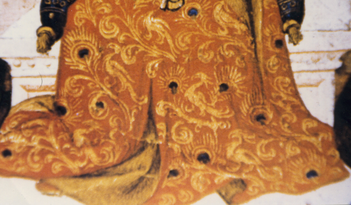
\includegraphics[width=8cm]{pics/fig27.png}
\caption[Franco-Flemish School: Prologue (detail)] 
{\it Franco-Flemish School: Prologue (detail), from the \textit{Livre de
Chasse} of Gaston Phebus, c. 1407.  Paris, Bib.~Nat., MS.fr. 616.}
\end{figure}
\begin{figure}[htbp]
\centering
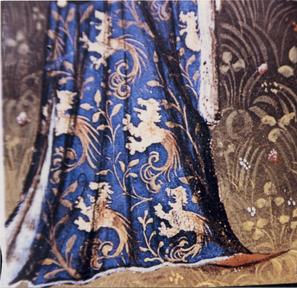
\includegraphics[width=8cm]{pics/fig28.png}
\caption[Franco-Flemish School: Training the Huntsmen (detail)] 
{\it Franco-Flemish School: Training the Huntsmen (detail), from the
\textit{Livre de Chasse} of Gaston Phebus, c. 1407.  Paris,
Bib.~Nat., MS.fr. 616.}
\end{figure}
from a Paris workshop, and stylistically close to
the Flemish Jacquemart de Hesdin, who worked for the Duc de Berry,
brother of Philip the Bold, from c.1380. A similar phoenix motif also
appears later in a section of the \textit{Tr\`es-Belles Heures de Notre
Dame}\footnote{Formerly in Turin, Royal Library (destroyed by fire);
see E. Panofsky, \textit{Early Netherlandish Painting}, op. cit. above
(note 26), Vol. Two, \textit{Plates}, Fig. 294: The Virgin Amongst
Virgins (the motif appears in the upper border of acanthus rinceaux -
the only case of substitution for the original borders executed for
the Duc de Berry).}, commissioned by the Duke and completed prior to
1417. Also, in all the lateral panels, the mantle of St.~Paul is
scattered with motifs in gold of summary fleurs-de-lys. These do not
necessarily have any heraldic significance. Studies have shown that
they sometimes served as a convenient `status symbol' used to
distinguish the important figure of a group.  I have found them used
in this way in a religious context in provincial Flemish
art\footnote{For example, in the Mus\'ee Municipale at Bastoigne
(Bastenaken), in present-day Belgium. A looser, more plant-like motif
does occur once in the copy of the \textit{Tacuinum Sanitatis} that
belonged to the Bishop of Trent; see J. Spencer, op. cit. above (note
55), p. 80, Livistichum (mountain celery). This, however, is a secular
context, and the subject requires further investigation.}.

Common to the main and the lateral panels is the geometric pattern
used for the podium, and for the floors of each interior.  This is a
version of a chequered design in which the squares are divided to form
triangles of alternating colour. The Mdina version, where the
triangles are set `on end' in vertical strips, is unusual in Italy,
but it does appear around 1400 for ceilings: in Lombard frescoes in
the border regions of the Alto Adige, and in embroidered panels
executed for Bishop George of Trent (which are listed in his inventory
as French) (Fig.29); 
\begin{figure}[htbp]
\centering
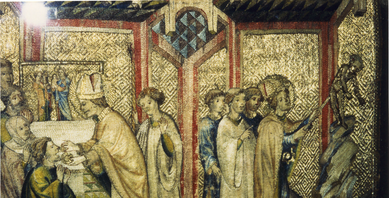
\includegraphics[width=10cm]{pics/fig29.png}
\caption[French School: embroidered panel, Scenes of the Life of St.~Virgil
(detail)] 
{\it French School: embroidered panel, Scenes of the Life of St.~Virgil
(detail), c. 1390-1407.  Trent, Museo Diocesano.}
\end{figure}
and in a recension of the \textit{Tacuinum
Sanitatis} now in Paris\footnote{Frescoes include those at Bressanone,
in the cathedral cloisters: for example, Arcade XI, dated 1400-1410,
The Emperor Charlemagne.  The embroidered panels, now in the Museo
Diocesano, Trent, depict scenes of the Life of S. Vigilio.  For the
Paris recension of the \textit{Tacuinum Sanitatis}, (Paris
Bib.~Nat. Nouv.~Acq. lat. 1673), see E. Pirani, \textit{Gothic
Illustrated Manuscripts, }London, 1970, Plate 39, The Tailor's
Shop.}. Also, the lack of any diminution in size in the Mdina pattern
as it `recedes' is consistent with most north European work until well
into the fifteenth century, and examples as a floor pattern identical
with the Mdina version come in miniatures by Flemish artists,
including Jacquemart de Hesdin, and a little later, sometimes with
slight diminution in size, by the Master of Gilbert of Metz and the
Master of Jean Mansel\footnote{For Jacquemart de Hesdin, see the
\textit{Tr\`es-Belles Heures de Jehan de France, duc de Berry} (`The
Brussels Hours'), Brussels, Bib.~Royal, MS. 11060/61, second dedication
page; illustrated in E. Panofsky, \textit{Early Netherlandish
Painting}, op. cit. above (note 26), Vol. Two, \textit{Plates},
Fig. 41. Regarding the Master of Gilbert of Metz see E. Panofsky,
loc. cit., Vol. One, \textit{Text}, p. 121 and note 9.  The Mdina
floor pattern is used in an illuminated Decameron of Boccaccio, Paris,
Bib. de l'Arsenal, MS. 5070; illustrated in E. Pognon,
\textit{Boccaccio's Decameron}, trans. J. Peter Tallon,
Fribourg-Geneva, 1978: e.g. Day IV--8, Neiphile by the Master of Jean
Mansel (p. 53), and Day IV--9, Philostrato by the Master of Gilbert
of Metz (p. 54).}.

Finally, an unusual feature of the throne of St.~Paul appears also to
derive from Flemish sources, namely the tall vertical shafts at
extreme left and right, with regularly-spaced, paired projections on
their outer edges. These represent, in outline, the architectural
framework that is typical of Flemish illumination of this period, as a
surround for sacred figures. Clear examples, with three-dimensional
mouldings and cornices in positions corresponding to the Mdina
silhouette, can be seen in miniatures attributed to Herman Scheerre,
an artist now identified with the `Herman of Cologne' who worked as an
assistant to Malouel at the Dijon court, from 1401--1403; also in
miniatures by his Flemish collaborator, known as the Master of the
Beaufort Saints\footnote{Both artists use the architectural framework
in the miniatures of the Beaufort/Beauchamp Hours, London,
BL. MS. Royal 2 A.,~XVIII; see R.~Marks and N.~Morgan, op.~cit. above
(note 60), Plate 31: Saint John of Bridlington (fol. 7v.) by the
Master of the Beaufort Saints; and Plate 32: The Annunciation
(fol. 23v.) attributed to Herman Scheerre.}. (Fig.30)
\begin{figure}[htbp]
\centering
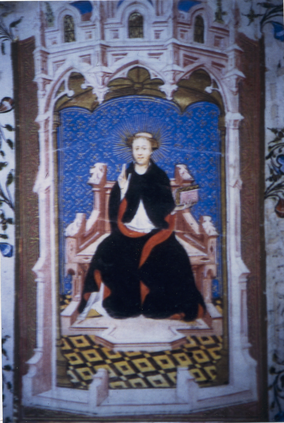
\includegraphics[width=5cm]{pics/fig30.png}
\caption[Master of the Beaufort Saints: St.~John of Bridlington] 
{\it Master of the Beaufort Saints: St.~John of Bridlington, from the
Beaufort / Beauchamp Hours, first decade of the fifteenth century.
London, British Library, Ms. Royal 2 A.XVIII, fol. 7v.}
\end{figure}


The upper section of the panel of St.~Paul Enthroned, that lies above
the Flemish type of architectural shafting just mentioned, combines
motifs used by Flemish and by Veneto artists. For instance, the acorns
seen in the design of the gold background are not common in Italy as a
decorative motif, and have patterning on the cup section that points
to Franco-Flemish work, such as the so-called M\'erode cup (Fig.31). 
\begin{figure}[htbp]
\centering
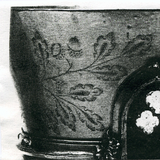
\includegraphics[width=5cm]{pics/fig31.png}
\caption[French School: The M\'erode Cup (detail)] 
{\it French School: The M\'erode Cup (detail), early fifteenth century.
London, Victoria and Albert Museum.}
\end{figure}
A
cup similarly decorated appears in the inventory of Jean Duc de Berry
in 1417\footnote{This covered beaker of the early fifteenth century
was originally owned by the ancient Belgian family of M\'erode, and is
now in the Victoria and Albert Museum, London; see (ed.)
P.~Williamson\textit{, The Medieval Treasury}, London, Victoria and
Albert Museum, 1986, illus. p.229 (detail), and text p. 228.}. The
leafy arabesques recall those found in the Calendar illustrations of
another Flemish work, the Hours of John the Fearless, Duke of
Burgundy, of 1406--15\footnote{Paris, Bib.~Nat., MS.lat.nouv. acq. 3055;
see J. Harthan, \textit{Books of Hours and their Owners}, London,
1978, no. 98, St.~Andrew (fol. 172v.) and no. 99, Pentecost
(fol. 28v.).}. At the same time, similar fleshy foliage does also
occur in the Veneto around 1400, and Guariento is one of several
artists who provide parallels for the characteristic strings of
`seedlings' that emerge in curvilinear fashion from open tulip-like
flowers amongst the Mdina foliage\footnote{For the foliage,
\textit{alla mano libera}, see a Venetian \textit{Portolano} (sea
chart), in Oxford, Bodleian Library, MS. Douce 390, illustrated in
catalogue: \textit{Italian Illuminated Manuscripts from 1400 to 1500},
Oxford, 1948, Plate I.  For the tulip-like flowers with `seedlings',
examples include Guariento's Virgin and Child of c.1338-45, now in the
Museo Civico, Padua; see B. Klesse, \textit{Seidenstoffe in der
italienscher Malerei des l4 Jahrunderts}, Bern, 1967,
Kat.~Nr. 161. Also in the region, are examples by Stefano da Zevio
(Stefano da Verona) in his Adoration of the Magi dated 1435, now in
the Pinacoteca Brera, Milan (the Virgin's mantle), illustrated in
S. Macioce, `Il gotico internazionale',\textit{Art e Dossier}, No. 34,
Rome-Milan, April 1989; by the much-travelled Taddeo di Bartolo
(documented 1386--1422), in a Virgin Lactans dated 1395, now in the
Hungarian National Gallery, Inv. No. 53,500 (decoration of predella
frame); and in ceiling decoration of the fifteenth century in Ferrara
(Via Palestro, 70).}.

Before proceeding to discuss further decorative features -- those that
come uniquely from the Veneto region -- it is useful to recall the
names of Semitecolo, Giusto de' Menabuoi and Altichiero, all of whom
have already been mentioned, particularly with reference to the
lateral panels. They belong to the generation after Guariento (who
gave the source for the throne of St.~Paul), and they all worked in
the Veneto. Zanino and Badile, whom we linked with the Mdina lateral
panels because of their use of a similar Franco-Flemish physiognomy,
also worked there and are included in this group. Others will be
identified, and are documented in Emilia and the Marches as well as in
the Veneto and Venice itself, and I shall refer to them occasionally
in abbreviated form as the `Veneto group'.

To return to the upper section of St.~Paul's throne, the complete
assembly of red pinnacles, large crockets, and finial can be ascribed
to prototypes in the Veneto, Emilia and the Marches. It is a design,
also, that has exact parallels in the monumental sculpture of Bologna
of the second half of the fourteenth century, and the close
interdependence of Bolognese and Venetian sculpture during this period
is well documented\footnote{See R. Grandi, `La scultura
tardogotica. Dai Masegne a Jacopo della Quercia', in catalogue (ed.)
R. Diamico and R. Grandi, \textit{Il tramonto del Medioevo a
Bologna. Il Cantiere di San Petronio}, Bologna, 1987, p. 127 ff., with
reference to further studies.  Amongst the memorial tombs of eminent
doctors of Bologna, that of Bartolommeo da Vernazza (died 1348), in
red Veronese marble, has crockets similar to those of the Mdina throne
of St.~Paul. The tomb is from the Church of St.~Peter, Bologna, and
now in the Museo Civico Mediovale, Bologna.}. The crockets, taken in
isolation, also feature in contemporary sculpture and in painting in
various other centres of Emilia and the Marches, as well as the
Veneto, being composed of acanthus leaves with a stubby, twisted
outline that is characteristic of this region.  In one such case, a
Trinity panel in Ferrara by the Master GZ, the stern, aulic frontality
of the figure of God-the-Father, and traces of prong-like
Veneto-byzantine highlights in the drapery, are additional features
that suggest an \textit{ambiente} similar to that of the Mdina
St.~Paul Enthroned.  This artist is considered, in fact, to be either
Veronese or Paduan, in the circle of Guariento's successor Altichiero,
and this work has been dated to c. 1380\footnote{The panel is now in
the Pinacoteca, Ferrara; see C.~L.~Ragghianti, op. cit. above (note
18), illus. 66 and illus. (in colour) p. 331. The Master GZ was
referred to above (note 22) in connection with a Ferrarese fresco
showing exterior domes above an interior scene. Other works featuring
the Mdina crockets are: the Trinity, a polyptic of 1360 by the Lombard
artist Turone, a work now in the Museo, Castelvecchio, Verona, best
illustrated in (ed.) R. Chiarelli and L. Magnato,
\textit{Castelvecchio e le Arche Scaligere}, Florence, 1969, Fig. 22
(detail: central panel); also a fresco fragment of a Virgin and Child
Enthroned from the Convent of San Francesco, Cesena, by the Master of
Castrocaro, of the end of the 14$^{th}$ or beginning of the 15$^{th}$
century, now in the Pinacoteca Comunale, Cesena (inv. n.226);
illustrated in the catalogue of the Pinacoteca, Cesena, 1984
n.2.}. (Fig.32) 
\begin{figure}[htbp]
\centering
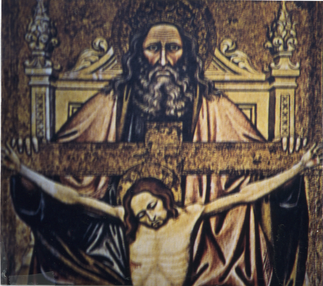
\includegraphics[width=8cm]{pics/fig32.png}
\caption[The Master GZ: The Trinity (detail)] 
{\it The Master GZ: The Trinity (detail), c. 1380.  Ferrara, Pinacoteca.}
\end{figure}
At this point it is worth noting that the method of
depicting the marble seat of the throne comes again from the same
\textit{ambiente}.  At this time there were several conventions in
painting for simulating marble: by packing the surface closely with
broad circular shapes; by covering it with painterly streaks of
colour; or as it appears here: small diamond and triangular patches of
colour set within a network of spidery diagonals. This pattern appears
in byzantine painting\footnote{For example, the marble columns in the
fresco of The Dormition of the Virgin, dated c.1265 at Sopocani,
Yugoslavia; see D. Tasic,\textit{ Byzantine Painting in Serbia and
Macedonia}, Belgrade, 1967, Fig. 23.}, and is not common in Italy, but
has a parallel in Semitecolo's Padua panel of \textit{St.~Sebastian
Encourages Two Christians}, dated 1367 (Fig.22), and (with more
regular reticulation) in miniatures from Ferrara now considered to
belong to the last years of the fourteenth century and attributed to
the Master of the Battuti Neri\footnote{The marble design by
Semitecolo is best illustrated in M. Prokopp, op.cit. above (note 50),
No. 45: St.~Sebastian Encourages Two Christians (the table leg in the
right alcove).  For the Master of the Battuti Neri, see miniatures of
the \textit{Libro della Confraternita dei Battuti Neri di Ferrara},
now in Venice, Coll. Vittorio Cini; illustrated in C.~L.~Ragghianti,
op. cit. above (note 18), Fig. l32: Resurrection of Christ.}.

A series of precise copies of Italian motifs is also to be seen in the
four lateral scenes, where some of the striking gold decoration is
recognisably different from the Franco-Flemish types identified above
on canopies, curtains and regal robes. The artist does not use
naturalistic foliage forms, either in loosely scattered sprays on
clothing, or densely packed for overall brocade effects.  Instead,
motifs on clothing (for example, the prelates' copes in the Baptism)
are more abstract, and include stylised rosettes and the form known as
`pineapple'; they are also placed in a regular pattern. The overall
design of the bed cover (in the Healing scene) uses the same motifs,
again in an ordered arrangement. These decorative features are
unquestionably of Italian origin. They are not unknown outside Italy,
but in such cases usually lack the tiny `commas' that form part of
each separate motif in the Mdina panels, and which seem to have
appeared in Italy from the late 1360s. As it happens, the detailed
analysis of Italian designs made by B. Klesse\footnote{B. Klesse,
op. cit. above (note 71).} enables the Mdina versions to be traced not
only to Italy, but to specific artists.  These artists all belong,
moreover, to the `Veneto group'. For instance, there are two types of
pineapple pattern in the lateral panels: in one the pear-shaped centre
section is reticulated, as in the Healing panel (the bedcover, Fig.7);
and in the other it is plain, as in the Baptism panel (the cope of
Ananias, Fig.33). 
\begin{figure}[htbp]
\centering
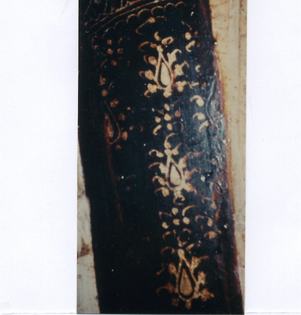
\includegraphics[width=5cm]{pics/fig33.png}
\caption[The Mdina retable of St.~Paul, lateral panel, The Baptism of
  St.~Paul (detail).]  
{\it The Mdina retable of St.~Paul, lateral panel, The Baptism of
  St.~Paul (detail).
The Cathedral Museum, Mdina, Malta. \copyright\ The Cathedral Museum,
  Mdina, Malta.} 
\end{figure}
Both types, equally surrounded by `commas', are used
by Semitecolo in his panel St.~Sebastian Encourages Two Christians
(Fig.22), already mentioned for his depiction of marble--a convention
also used in the Mdina panels.  Other artists of the `Veneto group'
who use the reticulated version include Semitecolo's collaborator in
Venice, Stefano Veneziano (\textit{plebanus} di Sant' Agnese), who was
also active in Friuli and Padua, as well as Ferrara; Marco Catarino,
who worked with Stefano; and Simone dei Crocifissi (documented 1355 -
c.1399), a Bolognese connected with Guariento in Venice (Figs.34 and
35). 
\begin{figure}[thbp]
\centering
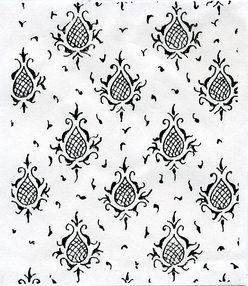
\includegraphics[width=5cm]{pics/fig34.png}
\hfill
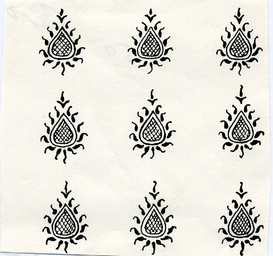
\includegraphics[width=5cm]{pics/fig35.png}
\hfill
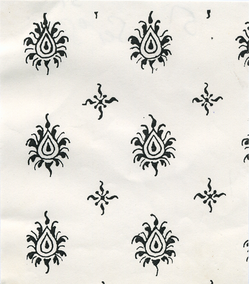
\includegraphics[width=5cm]{pics/fig36.png}
\caption[Stefano Veneziano: Virgin Enthroned with Saints, s/d 1385] 
{\it Stefano Veneziano: Virgin Enthroned with Saints, s/d 1385, Venice, San
Zaccaria; Caterino Veneziano: Coronation of the Virgin with Angels,
s/d 1375, Venice, Galleria dell'Accademia; Simone dei Crocifissi:
Coronation of the Virgin, s/d 1382, Bologna, Santa Maria Incoronata.
From B. Klesse, op.cit. above (note 71), Kat. Nr. 171.}
\caption[Caterino Veneziano: Madonna of Humility, c. 1380] 
{\it Caterino Veneziano: Madonna of Humility, c. 1380.  Baltimore, Walters
Art Gallery.  From B. Klesse, op.cit. above (note 71), Kat. Nr. 172.}
\caption[Serafino Serafini: Coronation of the Virgin, s/d 1384] 
{\it Serafino Serafini: Coronation of the Virgin, s/d 1384, Modena
cathedral.  From B. Klesse, op.cit. above (note 71), Kat. Nr. 173.}
\end{figure}
The plain version is used in the Vienna \textit{Tacuinum}, and by
the Modenese artist Serafino Serafini (c.1324--c.1393)
(Fig. 36).
\footnote{See B. Klesse, op. cit. above (note 71):
e.g. Kat. Nr.171.i (Stefano Veneziano), Kat. Nr.172 (Catarino),
Kat. Nr.171b (Simone) and Kat. Nr.173 (Serafino). For the Vienna
\textit{Tacuinum} see \textit{\"Osterreichische Nationalbibliothek,
Codex Vindobonensis, Series Nova}, 2644, fol. 104v. (tablecloth).}

Other features of gold decoration, relating to both technique and
design, again point to work of the `Veneto group'. One concerns the
gold striations used to heighten the tunic of St.~Paul in the
panels. These are not linked at intervals with ornamental cross-bands,
like many `byzantinising' striations in this region of Italy, but fill
an allotted area with plain rays from a single bar, or from a single
point, like those of Stefano Veneziano, Marco Catarino, and Donato (a
collaborator of Marco Catarino in the Marches as well as in
Venice). Also, the curvilinear form of the gold striations that fill
the lower drapery of St.~Paul in the Healing scene, and that are more
freely drawn than is usual, are a particular characteristic of work by
the latter two artists\footnote{For example, see R. Pallucchini,
op. cit. above (note 36), Fig.603 and Tav.~XXVII, The Coronation of the
Virgin, dated 1372, now in the Palazzo Querino Stampalia, Venice (the
lower folds of Christ's gown).}.

Finally, there is one feature common to all four scenes, and repeated
in the predella and the three upper panels with arched tops. This is
the design of the halos, an arrangement of quatrefoils on a stippled
ground.  Its use in isolation would be of little use as evidence,
because it appears widely in Italy. However, it does occur in works by
Simone dei Crocifissi of the Veneto group, and by other Bolognese
artists of the same period, and so represents a link of all these
subsidiary panels with Emilia. An Emilian source has already been
identified in the main panel, with reference to the red pinnacles,
crockets and finials. Emilian sources, therefore, emerge as a minor
unifying feature in a retable whose style we can now summarise as
follows: basically north Italian in conception, carried out by a team
of north Italian-trained artists (both traditional north-Italian and
courtly), working alongside others who followed Franco-Flemish models.


\subsection{\textit{The Upper Register}}

The same elements can readily be identified in the rest of the
retable, and we may begin with the panel of the Virgin and Child
which, with the predella panels, is `traditional Veneto'. In one
respect, the style of the two central figures, the composition is
\textit{retardaire}.  That is to say, the underlying iconography of
the Virgin and Child reflects back to a tradition of the
mid-fourteenth century that survives in Verona churches in frescoes
attributed to the so-called `Second Master of San Zeno'. The Virgin's
unbending stance and general lack of affectivity, the scroll held by
the Child, and the position of His slightly splayed-out legs, are all
part of this older tradition\footnote{See E. Sandberg-Vaval\`a,
\textit{La Pittura Veronese del Trecento e del primo Quattrocento},
Verona, 1926, especially Chapter IV, where all these features are
illustrated.}. Quite within the limits of this basic formula, the
drapery of the Virgin's voluminous mantle provides an immediate link
with the main panel, in that its stylised byzantine modelling, wide
arabesques accentuated by a heavy gold border, and scattering of
Franco-Flemish motifs, all mirror that of St.~Paul. There are
reflections in the sweep of this drapery of the most illustrious of
all the artists working in Venice around the turn of the century:
Gentile da Fabriano (c.1370--1427)\footnote{Comparisons can be drawn
from the following early works: The Valle Romita polyptic, now in the
Brera Gallery, Milan; and the Virgin and Child with Two Angels, now in
the Philbrook Art Centre, Tulsa (Oklahoma); see \textit{L'Opera
Completa di Gentile da Fabriano}, op.cit. above (note 53), Tav. III
and Tav. XIV respectively.}. Recent scholarship has suggested, in
fact, that Gentile, while engaged on the second stage of the
decoration of the Sala del Maggior Consilio, had members of the
`Veneto group' working with him\footnote{Artists of the `Veneto group'
possibly working with Gentile on the Sala paintings include Jacobello
del Fiore, Michelino da' Besozzo and Zanino; see P. Fortini Brown,
op. cit. above (note 34), p. 246, note 41. Gentile was the recipient
of high honours by the Venetian Senate by 1408, and remained in Venice
until 1414.}. There are other features of this panel clearly
associated with the group: the Lombard physiognomy of both Virgin and
Child is seen in female heads by artists of the circle of Altichiero,
and by Veronese artists of the following generation, including Stefano
da Verona (c.1375--1451), who also occasionally imprinted facial
features with the peculiarly circumspect expression that characterises
the Mdina Virgin, as well as female figures elsewhere in the
retable. Again, the fact that the crowned Virgin wears no veil, or
other vestige of the byzantine maphorion, usually indicates a northern
artist, and this type was favoured increasingly in north Italy by the
turn of the century: Michelino da Besozzo, of the `Veneto group'
(active Pavia and Milan 1388--1415), a prestigious Lombard court
artist documented with Gentile just after 1400, is a case in
point. Finally, angel musicians accompanying a Virgin \textit{Assunta}
were not a novelty by this time, and Guariento and artists of the
`Veneto group', Stefano Veneziano and Jacobello del Fiore, all include
angels playing the same versions of the shawn, portative organ, viol
and lute. These instruments also appear in the \textit{Tacuinum
Sanitatis} ascribed to the workshop of Giovanino de' Grassi -- our
important source for the courtly companions of St.~Paul in the Healing
scene.

The two other upper panels with arched tops, the Road to Damascus and
the Miracle of the Viper (Figs. 37 and 38), 
\begin{figure}[htbp]
\centering
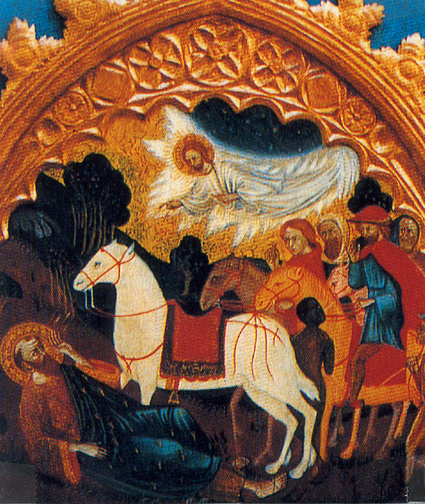
\includegraphics[width=8cm]{pics/fig37.png}
\caption[The Mdina retable of St.~Paul, The Road to Damascus] 
{\it The Mdina retable of St.~Paul, The Road to Damascus.  
The Cathedral Museum, Mdina, Malta. \copyright\ The Cathedral Museum,
  Mdina, Malta.} 
\end{figure}
\begin{figure}[htbp]
\centering
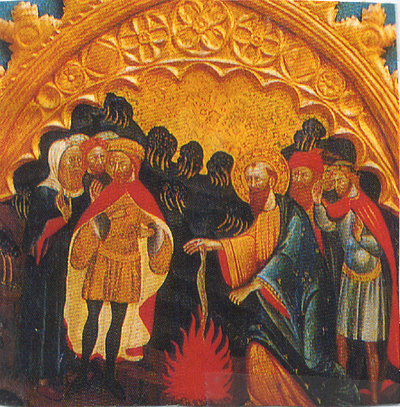
\includegraphics[width=10cm]{pics/fig38.png}
\caption[The Mdina retable of St.~Paul, The Miracle of the Viper] 
{\it The Mdina retable of St.~Paul, The Miracle of the Viper.  
The Cathedral Museum, Mdina, Malta. \copyright\ The Cathedral Museum,
  Mdina, Malta.} 
\end{figure}
also feature the courtly
figures of this same \textit{Tacuinum}. In the Road to Damascus, in
fact, St.~Paul is accompanied across country by a cavalcade, and
watched by a passing countryman, all familiar from \textit{Tacuinum}
scenes of the courtly country life of the Padana. The inclusion of a
black servant, seen here against the neck of the brown horse,
emphasises the grandeur of courtly life, and is not rare (for instance
in scenes of the Three Magi): artists of the `Veneto group' from
Altichiero onwards furnish several examples\footnote{For example,
Altichiero, in the Beheading of St.~George, a scene in the cycle of
frescoes by Altichiero and other artists in the Oratory of St.~George,
Padua, of c.1377--84. (This particular scene is attributed to
Altichiero himself.) A black servant is also included by Jacobello del
Fiore (alluded to above, note 17) in his Adoration of the Magi, now in
the National Museum Stockholm; illustrated in \textit{Il Gotico
Internazionale in Italia}, op.cit. above (note 52), Doc.4.}. The fact
that the Limburg brothers, in an illumination in the Tr\`es Riches
Heures of the Duc de Berry, show a black servant in the same
contrapposto attitude, may indicate a common model\footnote{Fol.51v;
now in the Mus\'ee Cond\'e, Chantilly, France; illustrated in \textit{Les
Tres Riches Heures du duc de Berry}, trans. D.~Macrae, Mus\'ee Cond\'e,
n.d. The scene is the meeting of the Three Magi at the crossroads near
Golgotha--a scene unknown before the very end of the 14$^{th}$
century; see E.~Panofsky, \textit{Early Netherlandish Painting},
op.cit. above (note 26), vol. One, \textit{Text}, p.64 and note 4. It
should be noted here that constant traffic between one centre of
patronage and another--in this case between the Limburgs in Dijon and
the Visconti workshops--has sometimes led to disagreement as to the
place of origin of an image.}. (c.f. Figs.37 and 39)
\begin{figure}[htbp]
\centering
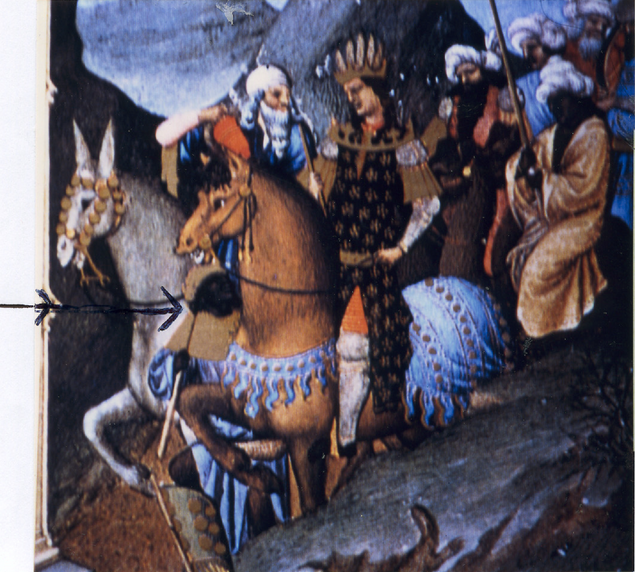
\includegraphics[width=10cm]{pics/fig39.png}
\caption[The Limburg Brothers: The Meeting of the Three Magi (detail),
  from \textit{Les Tr\`es Riches Heures} of the Duc de Berry, c. 1411-
  c. 1416]  
{\it The Limburg Brothers: The Meeting of the Three Magi (detail),
  from \textit{Les Tr\`es Riches Heures} of the Duc de Berry, c. 1411-
  c. 1416. Chantilly, Mus\'ee Cond\'e.}
\end{figure}


In the Viper panel St.~Paul's low forward lunge is again the trademark
\textit{par excellence} of \textit{tacuinum} men and women as they
engage in their different country pursuits\footnote{For many examples
of the forward-thrusting stance in the \textit{Tacuinum Sanitatis} of
Bishop George see (ed.) J. Spencer, op.cit. above (note 55).}
(Fig.26); on the other hand his stance may come from an ancient
prototype\footnote{One such prototype stylistically close to the
St.~Paul figure in the Viper scene would have been a scene in the
fresco cycle of the Lives of St.~Peter and St.~Paul in the Church of
S. Paolo fuori le Mura, Rome, of c.1278-9. In many cases these frescos
were a repainting of an earlier fifth century cycle; they were
destroyed by fire in 1823, but are known from seventeenth century
copies; see S. Waetzoldt, \textit{Die Kopien des l7. Jahrhunderts nach
Mosaiken und Wandmalereien in Rom}, Rome, 1964, Fig. 406. A later
example, but less close stylistically to the Mdina version, is the
fresco fragment in Canterbury Cathedral (St.~Anselm's Chapel, north
wall) of c. 1150--1175; see J. Azzopardi, `St.~Paul's Malta Shipwreck
in Art', in (ed.)  J.~Azzopardi, \textit{St.Paul's Grotto, Church and
Museum at Rabat, Malta}, Malta, 1990, p.481; see also O. Demus,
\textit{Romanesque Mural Painting}, London, 1970, p.509 and Plate
p. 121.}. The secular costumes, like those in the Healing panel, have
parallels in miniatures attributed to Altichiero and his
circle\footnote{For example, the Darmstadt \textit{De Viris
Illustribus} (see above note 46), and a Paduan Bible of c.1400:
Rovigo, Accademia dei Concordi, MS.212, illustrated in Pallucchini,
op.cit. above (note 36) Fig.470. For an example of the round hat of
Publius being worn by a French dignitary, see the sculpture of Jean
Bureau de la Rivi\`ere on the exterior of Amiens cathedral (north tower)
of the end of the fourteenth century; illustrated in (ed.) R.~Huyghe,
\textit{Larousse Encyclopedia of Byzantine Medieval Art}, London,
1974, illus.832.}, being French styles common to northern courts:
Publius in the Viper scene, for instance, is a mirror-image of a
sculpture of Casimir the Great (1370--1380) now in the Gothic Museum,
Cracow. (Fig.40) 
\begin{figure}[htbp]
\centering
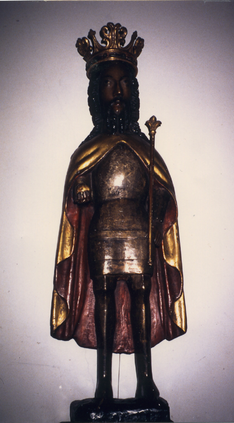
\includegraphics[width=4cm]{pics/fig40.png}
\caption[Casimir III `The Great', sculpture dated c. 1370-80] 
{\it Casimir III `The Great', sculpture dated c. 1370-80.  Cracow, Gothic
Museum.}
\end{figure}
Again, a Veneto-byzantine element is indicated by
some barely detectable byzantine modelling (notably for the standing
figure on the extreme left of the Viper scene), and by the pinched
physiognomy of St.~Paul, with oversized cranium, associated with the
`byzantinising' art of the region of the Veneto.

The artist responsible for the rural backgrounds of these two scenes,
on the other hand, has followed a well-attested Franco-Flemish design:
a traditional arrangement found in fact in all the Franco-Flemish
miniatures we have already cited as sources for Franco-Flemish
features elsewhere in the retable (fringed canopies, decorative sprigs
and phoenix and dragon motifs). It is a landscape in which trees of
various types are always inserted without regard to their natural
size, and are smaller within the lower zone so as not to obscure the
action of the figures placed on the first `ledge', where the action
takes place. The key to the specific source of the Mdina design lies
in the particular form of the clumps of trees: bearing yellow and
orange fruit, these trees are tightly bunched together with their
slender trunks curving in parallel. Such clumps feature in miniatures
executed for Giangaleazzo Visconti (d.1402) and attributed to artists
of the `Veneto group', Michelino da Besozzo and Giovannino de' Grassi,
and, a little later, to Belbello da Pavia (Fig.41). 
\begin{figure}[htbp]
\centering
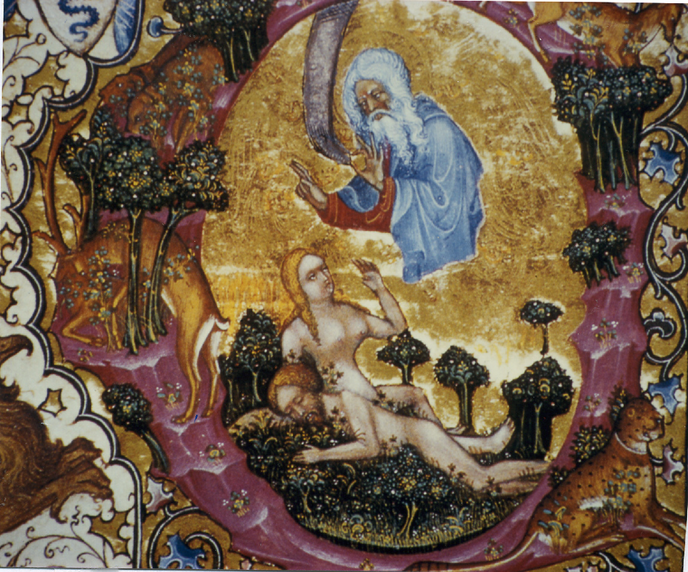
\includegraphics[width=10cm]{pics/fig41.png}
\caption[Belbello da Pavia, The Creation of Eve (detail), from the Visconti
Hours,(second stage), c. 1428] 
{\it Belbello da Pavia, The Creation of Eve (detail), from the Visconti
Hours,(second stage), c. 1428.  Florence, Bib.~Naz. Ms. LF.22,
fol. 46v.}
\end{figure}
With features in the other narrative panels so clearly traceable to
the Visconti workshops, this comes as no surprise. The ultimate source
for the style lies in illuminations attributed to the so-called
`Ma\^itre aux Boquetaux' (lit. `little clumps'), for example, The
Hours of Philip the Bold, Duke of Burgundy, of c.1370. He worked in
the influential Paris workshop of Jean Bondol (John of Bruges, active
Paris 1367--c.1381). It was Bondol's interest in creating
naturalistic three-dimensional landscape that produced the arrangement
of step-like ledges to give depth, punctuated by trees in little
clumps that often resembled overgrown mushrooms or umbrellas. A series
of prestigious manuscripts flowed from this workshop, commissioned by
all the wealthy patrons of the day, and the landscape style was widely
imitated.

These backgrounds later underwent a striking transformation: sweeping
changes that brought the landscapes right into line with the latest
theories being worked out first in Dijon and then in Venice just after
the turn of the century\footnote{Whether the changes were made by
order of the patron who originally commissioned the retable, or later
at the suggestion of a new owner, need not concern us here; narrative
paintings not infrequently had features of landscape inserted at
various times after their initial execution.}. (Figs.42 and 43) 
\begin{figure}[htbp]
\centering
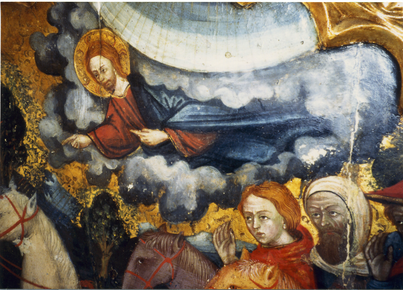
\includegraphics[width=8cm]{pics/fig42.png}
\caption[The Mdina retable of St.~Paul, The Road to Damascus: overpainting
(detail)] 
{\it The Mdina retable of St.~Paul, The Road to Damascus: overpainting
(detail).  Mdina, Malta, Cathedral Museum.}
\end{figure}
\begin{figure}[htbp]
\centering
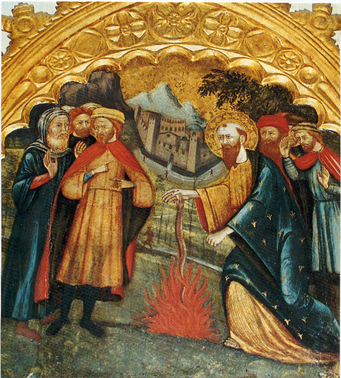
\includegraphics[width=8cm]{pics/fig43.png}
\caption[The Mdina retable of St.~Paul, The Miracle of the Viper: overpainting
(detail)] 
{\it The Mdina retable of St.~Paul, The Miracle of the Viper: overpainting
(detail).  Mdina, Malta, Cathedral Museum.}
\end{figure}
The
extensive overpainting was removed recently when the panels were
cleaned, but the photographic record provides ample evidence of these
innovations, pointing unmistakably in fact to the influence of
Gentile da Fabriano, who was working in Venice until 1414. It is worth
pointing out the most significant changes.

The earliest exponents of these important developments were Flemish,
and a \textit{terminus post quem} of c.1394 for the overpainted Mdina
landscapes is provided by panel paintings by Melchior Broederlam of
Ypres, a contemporary at the Dijon court of Claus
Sluter\footnote{Broederlam's panels decorate the external wings of a
celebrated carved altarpiece, paid for in 1394 and installed at the
Chartreuse de Champmol in 1399, and now in the Mus\'ee de Beaux Arts,
Dijon. See especially the Annunciation and Visitation, also the
Presentation of Christ in the Temple and Flight into Egypt,
illustrated in E.~Panofsky, \textit{Early Netherlandish Painting},
op. cit. above (note 26), Vol. Two, \textit{Plates}, Fig.104 and
Fig.105. For Claus Sluter, and the spread of a new Franco-Flemish
figure style, see above (Section II and note 38).}, a sculptor already
linked stylistically to the retable in connection with the robust
`elders' of the lateral scenes. In the interests of recession the
Mdina artist, like Broederlam, used an oblique perspective for
buildings when these were shown isolated in a landscape. Also, the
artist inserting a city in the Viper panel took the ancient polygonal
format, in `bird's eye view', masking the furthest walls with the
city's interior buildings, and showing the forward sections of wall in
elevation. Studies on this subject have shown that by 1430, after a
relatively short experimental period, this particular perspective for
a distant city seems to have disappeared from all the more important
centres of the West\footnote{For a wider treatment of the
representation of cities, see A. Cutler, `Forma Urbis', in
\textit{Transfigurations; Studies in the Dynamics of Byzantine
Iconography}, Pennsylvania State University, 1975, p. 122ff.}.

Broederlam's contemporary Gentile da Fabriano was amongst the Italian
artists who took up the same system for landscapes.  His contacts with
a court painter to the Duke of Burgundy during the opening years of
the fifteenth century, as well as with members of the `Veneto group',
are documented. Though few paintings from Gentile's early period in
Venice and in Brescia have survived, the landscapes in his altarpiece
of the Adoration of the Magi of 1423 have many details that are
repeated in the overpainted Viper panel: for example, the centre panel
of Gentile's predella has similar naturalistic mountains (steep, with
flattened tops and colour differentiation, and soft modelling), as
well as a city with rectangular towers, and, within its walls,
blue-domed buildings\footnote{See \textit{L'Opera Completa di Gentile
da Fabriano}, op. cit. above (note 53), Tav. XXXVI--XXXVII and
Tav. XXXVIII, The Flight into Egypt.}.  Here again, his country house
with gabled roof and arched doorway, just outside the city walls, was
repeated in this scene, behind the figure on the extreme left of the
panel. Similar architecture is also seen in more ornate versions by
the Limburg brothers, two of whom were employed at the Dijon court
from 1402. Most important of all, although a few `boquetaux' were
still discernible, the land mass as a whole became a series of shallow
overlapping curves in carefully varied shades of green, giving the
impression of vast gently undulating meadowlands. Trees and mountains,
placed in opposition at the margins of the Viper scene served as
`coulisses' for the central, more distant view, and buildings and
distant figures were shown in appropriate sizes along a series of
winding pathways. Gone were the tiny foreground trees, to be replaced
by a scattering of small plants reminiscent of the flowered meadows
beloved of Gentile.

It is worth noting that the device of placing small figures along
winding pathways that became standard practice in this new
organisation of landscape, sometimes merely involved a few touches of
red sinopia, as in the repainted panels.  Red sinopia was used, for
example, by Antonello da Messina, who acquired Flemish techniques
before his visit to Venice in 1475, and in his case through contacts
with Flemish artists at the Angevin court in Naples\footnote{For
example, in his Crucifixion, signed and dated 147-(sic), now in the
National Gallery, London; see M. Lucco (ed.), \textit{Antonello da
Messina, L'Opera Completa}, Milan,2006, pp. 184--5, where the precise
date is fully discussed.
%\textit{Landscapes}, National Gallery Diary, 1985, October 21-27.  The
%date is disputed (1475 or 1477), but evidence suggests that this work
%post-dates his Naples period.
}. The same device appears as one of the hallmarks of the Italianate
landscapes that came to be inserted as background in paintings in
Crete, and in Cyprus, while these islands were under Italian
influence\footnote{For example, a Cretan icon of Christ and the
Samaritan Woman of 1475-1480, now in Athens, Byzantine Museum, T. 737;
see exhibition catalogue, \textit{From Byzantium to El Greco, Greek
Frescoes and Icons}, London, Royal Academy, 1987, Plate 50, and text
by N. Chatzidakis, p. 181-182, with bibliography. This landscape also
includes, not far from the city walls of Samaria, the small house of
Gentile's Flight into Egypt. In Cyprus examples are found in frescoes
attributed to the Italo-byzantine school, dated c. 1500, in the
so-called `Latin Chapel' of the Monastery of St.~John Lampadistis,
Kalopanayiotis; see A.~and J.~A.~Stylianou, op.~cit. above (note 12),
especially Fig. 88, Moses receiving the Ten Commandments, and
Fig. 189, Moses and the Vision of the Burning Bush (frescoes in the
apse, left and right spandrels respectively).}.

The developing realism did not extend to the sky, which remained gold,
as in all Gentile's early works, and the hovering figure of Christ
kept the red hair and facial features that merely repeat those of
St.~Paul's companions below (Fig.42). On the other hand, He emerges
from a swathe of convoluted clouds, beneath a carefully delineated
segment of the `dome of Heaven' with its golden rays. The clouds are
of particular interest, because they mark a transition in style: their
basic formation harks back to stylised Romanesque models seen all over
northern Europe and Northern Italy (the Alto Adige, for
example)\footnote{Examples in the Alto Adige include the fresco cycle
at Riffiano of 1415 by Meister Wenzeslaus, a Bohemian artist already
cited above, Section II, for his figural style. For Guariento, see the
stylised clouds beneath the feet of a group of Principalities in a
panel from the Cappella Carrarese, Padua, attributed to Guariento and
dated to the 1350s (now in the Museo Civico, Padua); illustrated in
R.~Pallucchini, op.cit. above (note 36).}, but their execution was now
painterly, and naturalistic in effect.

Finally, the number of bare trees dispersed in the new Viper landscape
deserves a mention. Bare trees had a symbolic function, to signal a
stark mood but also eventual rebirth. They were prominent in Flemish
miniatures from the Bondol workshop and occur in paintings by
Guariento and by Gentile\footnote{For Guariento, the bare tree appears
in The Vision of St.~Augustine, part of a fresco cycle now unanimously
attributed to Guariento and dated 1360-1365, in the Church of the
Eremitani, Padua (left wall of presbytery); see F.~F.~D'Arcais,
\textit{Guariento}, op.cit. above (note 15), Fig. 100.  For Gentile,
the predella of his altarpiece The Adoration of the Magi, left panel,
The Nativity (Joseph sits apart under a bare tree); see
\textit{L'Opera Completa di Gentile da Fabriano}, op.cit. above (note
53), Tav. XXXIX A.}.  By about 1400, however, landscape was sometimes
given a seasonal aspect (an early Italian example can be seen in the
Rome recension of the \textit{Tacuinum Sanitatis}), and such may be
the case in both these overpainted panels, the feast of the Conversion
of St.~Paul being celebrated in both East and West on January
25$^{th}$; and the `Miracle of the Viper' having taken place around a
fire, kindled ``because it had begun to rain and was
cold''\footnote{Acts 28.2.}.

The design incised on the gold backgrounds of these two panels
establishes links with both St.~Paul Enthroned and the central panel
of the predella. (Fig.44) 
\begin{figure}[htbp]
\centering
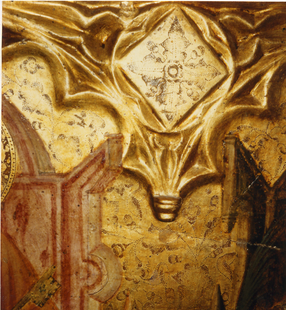
\includegraphics[width=8cm]{pics/fig44.png}
\caption[The Mdina retable of St.~Paul, predella (detail).]  
{\it The Mdina retable of St.~Paul, predella (detail).  
The Cathedral Museum, Mdina, Malta. \copyright\ The Cathedral Museum,
  Mdina, Malta.} 
\end{figure}
This appears to have a northern source, in
that it includes daisy-like flowers that are seen in English
illumination, including some border decoration in a group of
manuscripts of the early 1380's now at Westminster Abbey, London, as
well as those of the Master of the Beaufort Saints, already quoted for
architectural framework for figures that is identical to that of the
Mdina St.~Paul Enthroned (c.f. Fig.30)\footnote{Examples are in the
\textit{Liber Regalis} of ?1382, London, Westminster Abbey MS. 38,
e.g.~fol.20: The Coronation of a King and Queen; and in the English
Lytlington Missal, London, Westminster Abbey Ms. 37 of 1383-4
e.g.~Vol.II, fol.~157 v.: The Crucifixion; see R.~Marks and N.~Morgan,
op. cit. above (note 60), Plates 24 and 25 respectively.}. In the
diamond-shaped decoration that fills the spandrels of the frame of the
Mdina predella (Fig.44) similar flowers form a design seen on
line-impressed tiles of the fourteenth century, found in England, that
may be French\footnote{See E. Eames, \textit{English Medieval Tiles},
British Museum, London, 1985, no. 34; also E.~Eames, \textit{English
Tilers}, British Museum, London 1992, no.25.}. Furthermore, on some
tiles in the same collection the flower motif is replaced by an acorn,
with the Franco-Flemish patterning as acorns already identified in the
gold background of St.~Paul Enthroned (Fig.45). 
\begin{figure}[htbp]
\centering
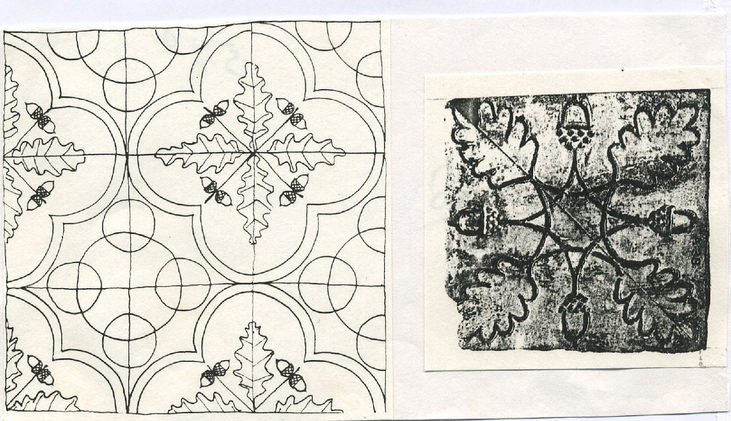
\includegraphics[width=10cm]{pics/fig45.png}
\caption[French(?) line-impressed tiles, fourteenth century] 
{\it French(?) line-impressed tiles, fourteenth century.  London, British
Museum.}
\end{figure}
However, in addition
to all this evidence for a northern design, the Mdina flowers also
occur occasionally in Emilian illumination, including a miniature now
attributed to the Compagno Ferrarese, an artist already mentioned in
connection with the architectural setting of the Healing panel, and in
some illuminated \textit{corali} in Ferrara\footnote{For the Compagno
Ferrarese, see above Section II and note 22. For the flowers in a
miniature attributed to the Compagno Ferrarese, see the dedication
page of the \textit{Historia Angliae} by Galasso, dated 1442 (Paris,
Bibliotheque Nationale, MS. lat. 6041), illustrated in
C.~L.~Ragghianti, op. cit. above (note 18), illus. 224. For similar
versions of the flower see also \textit{Libro Corale K} of 1400-1450,
from the Convent of San Giorgio, Ferrara, now in the Palazzo
Schifanoia, Ferrara.}. The design on the gold backgrounds of the upper
panels and the predella also share a technique usually considered
northern and similarly seen in Emilia during the same period: motifs
are composed of strings of tiny `dots', incised with a small metal
roller\footnote{Examples include the decoration of a polyptic of the
Virgin and Child and Saints by Antonio di Carro (documented in
Piacenza 1392-1410), now in the Mus\'ee des Arts Decoratifs, Paris; see
catalogue, ed. M. Laclotte, op.cit. above (note 10), No. l6; also a
panel of St.~George by the Maestro delle Storie di Elena (stated to be
`of the Veneto', active 1440-70), now in the Pinacoteca, Ferrara.}. In
conclusion, it is clear that Italy cannot be ruled out as a source for
the subsidiary decoration in both upper panels and predella. It is as
eclectic as the background to St.~Paul Enthroned, which was also seen
to include features found in more than one milieu.

\subsection{\textit{The Predella}}

Many features of the predella panels combine to support the general
designation `traditional Veneto', and in the case of the left and
right hand panels, two irrefutable sources are particularly helpful.
Most notable of these is the sarcophagus in the scene of the
\textit{Veneration at the Tomb of St.~Paul} (Fig.46). 
\begin{figure}[htbp]
\centering
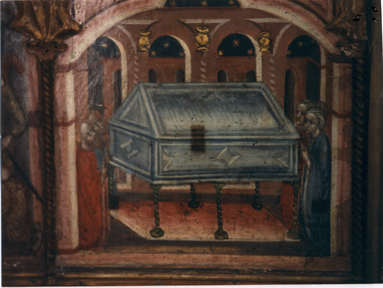
\includegraphics[width=10cm]{pics/fig46.png}
\caption[The Mdina retable of St.~Paul, The Veneration at the Tomb of
  St.~Paul]  
{\it The Mdina retable of St.~Paul, The Veneration at the Tomb of St.~Paul.
The Cathedral Museum, Mdina, Malta. \copyright\ The Cathedral Museum,
  Mdina, Malta.} 
\end{figure}
It has a distinctive structure (see Points of Iconography, Addendum,
p.~8 above) also found
%%%%particularly associated with Verona and Padua, and it appears
in dated works by two artists of the `Veneto
group' already mentioned 
%%%%%as the source of various features 
for their use of other features seen
%
in the Mdina panels: Semitecolo and Gentile da Fabriano. For instance,
there are two similar sarcophagi in one of Semitecolo's panels in
Padua of 1367: in the scene of \textit{The Burial of St.~Sebastian}
they are placed high on their special marble plinths in the apses of
adjoining side chapels\footnote{See \textit{Paolo Veneziano e Il Suo
    Tempo}, op. cit. above (note 30), Tav. X.} (Fig.12).  Gentile's
version is perhaps better known: it dominates his Washington panel of
1425: \textit{A Miracle of St.~Nicholas}, high focal point for the
lame and sick as they ascend the sanctuary steps to touch the tomb of
the saint\footnote{This panel, now in the National Gallery,
  Washington, formed part of the predella of his signed Quaratesi
  polyptic of 1425, dismantled in the 19$^{th}$ century. In Italian
  the scene is usually given its full title: \textit{Infermi e
    pellegrini alla tomba di San Nicola}; see \textit{L'Opera Completa
    di Gentile da Fabriano}, op. cit. above (note 53), Tav. LIX.}.

The Venetian feature in the panel of the Sea Voyage is a small detail,
but nevertheless informative: it concerns the unusual double anchor,
attached to a single ring, drawn up against the prow of the boat.
This type, with curved-back prongs and extra long shanks appears in a
Venetian watermark of 1376\footnote{See F. Moll, \textit{Das Schiff in
der bildenden Kunst}, Bonn, 1929, Fig. E.II.g.}.

On the question of dating, once more the paintings of Altichiero and
his followers and the artists of the `Veneto group' provide many of
the sources. In Altichieran miniatures are found, not only the
sarcophagus of the Veneration, but features of the Sea Voyage: the
painterly, rounded waves, the Roman official in corium and winged
helmet\footnote{In addition to the Milan \textit{Titus Livius} cited
above (note 47), see the miniatures of the Paris \textit{De Viris
Illustribus} of 1380, Paris, Bib.~Nat., MS. lat.6069G, in Pallucchini,
op.cit. above (note 36), Fig.479.}. The left-hand coastline is a
design used by Giusto de' Menabuoi in his cycle in the baptistery of
Padua cathedral (Fig.47), 
\begin{figure}[htbp]
\centering
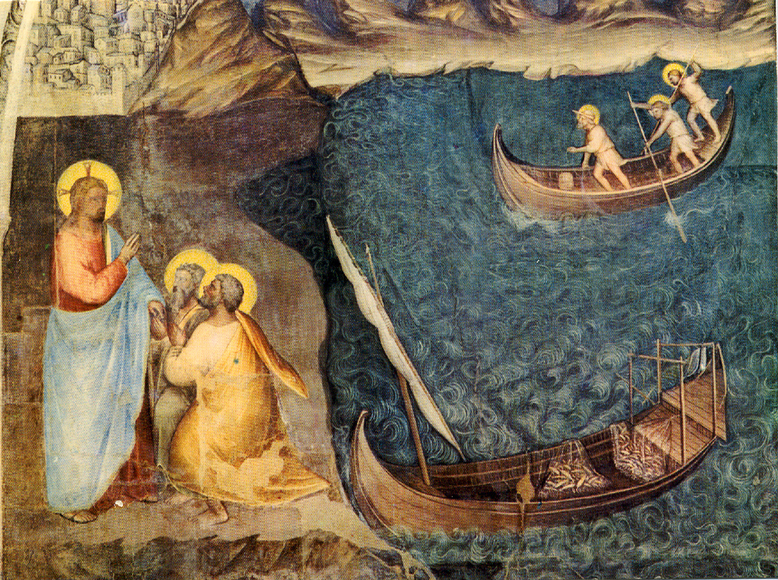
\includegraphics[width=10cm]{pics/fig47.png}
\caption[Giusto de'Menabuoi: The Calling of Andrew and Simon Peter,
  mid. 1370s]  
{\it Giusto de'Menabuoi: The Calling of Andrew and Simon Peter, mid. 1370s.
Padua Cathedral, Baptistery.}
\end{figure}
a design which itself has an earlier source
in Ambrogio Lorenzetti\footnote{Giusto's sea scene in the baptistery
cycle, Padua cathedral, is The Calling of Andrew and Simon Peter.  For
Ambrogio Lorenzetti's prototype, see part of his Pala di S. Procolo
(lower scene), illustrated in E. Carli, \textit{I Lorenzetti}, I
Maestri del Colore, No. 71, Milan, 1965, Tav. X.}; it has been
repeated, neatly reversed on the right hand side of the Sea Voyage, to
provide the shore of the island of Malta.

The disparity between the two separate scenes making up the left hand
predella panel is emphasised by their different diaphragm arches.
That of the Veneration on the right is a Venetian trefoil arch,
consistent with the Veneto sarcophagus. The composition of the
Beheading scene has been organised, on a smaller scale, to match the
matrix of the four lateral scenes, and its horizontal diaphragm is not
dissimilar to that of the Healing panel, and has the same diaper
pattern inserted above it. Also, St.~Paul's gown in this panel has a
version (with finer detailing) of the Flemish phoenix motif that was
identified in the curtain design of the Healing (Fig.48). 
\begin{figure}[htbp]
\centering
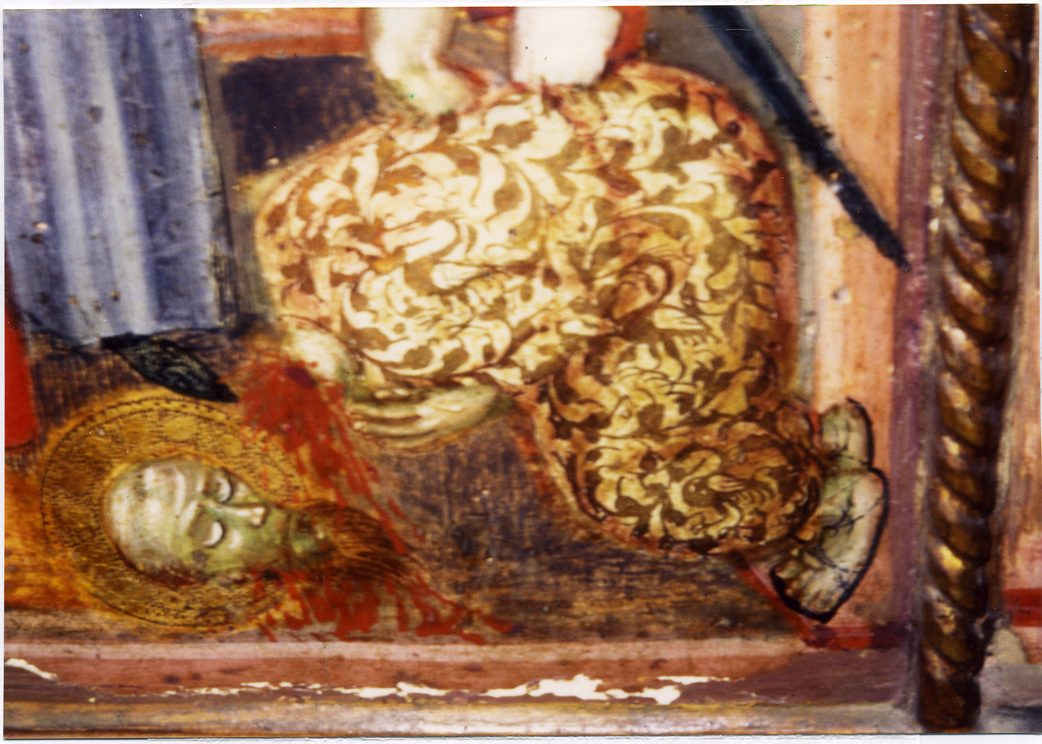
\includegraphics[width=10cm]{pics/fig48.png}
\caption[The Mdina retable of St.~Paul, The Beheading of St.~Paul (detail)] 
{\it The Mdina retable of St.~Paul, The Beheading of St.~Paul (detail).
The Cathedral Museum, Mdina, Malta. \copyright\ The Cathedral Museum,
  Mdina, Malta.} 
\end{figure}
The scene
also includes the \textit{poulaines}, and a Flemish fringe for the
canopy over the throne. At the same time it is interesting to note
that, amongst the Emperor's entourage, the two central figures, by
their dress and gestures, appear to represent Bolognese lawyers
(Fig.49)\footnote{From the time of the official foundation of Bologna
University in 1343, doctors of civil law wore scarlet, and doctors of
canon law wore blue; the latter sometimes wore a turban-like cap,
similar to the Mdina figure in blue. In the Beheading scene both these
figures appear, by their explicit gestures, to accept the sentence
passed (the open hand), and even, in the case of the figure in
scarlet, to re-enforce this (the pointing finger).}.
\begin{figure}[htbp]
\centering
\includegraphics[width=10cm]{pics/fig49.png}
\caption[The Mdina retable of St.~Paul, The Beheading of St.~Paul (detail)] 
{\it The Mdina retable of St.~Paul, The Beheading of St.~Paul (detail).
The Cathedral Museum, Mdina, Malta. \copyright\ The Cathedral Museum,
  Mdina, Malta.} 
\end{figure}

In one notable respect both these predella interiors differ from the
lateral scenes: they show a more advanced understanding of
perspective. In both, the arrangement of the arcading produces a
deeper space that is less ambiguous.  The Veneration goes further, in
having `two-room recession'; also, a marble plinth with convincing
perspective and naturalistic lighting replaces the
vertically-patterned floor tiles of the lateral scenes. From what is
known of workshop organisation and practice, however, stylistic
differences of this order do not necessarily infer a different date,
nor even a different artist.

In the final panel to be examined, the central component with its
three enthroned saints, it is a question of `the mixture as before';
that is to say, as identified throughout our survey of the central
section of the retable: Lombard and Venetian, and again a Flemish
contribution and possible references to Emilia.

In the first place, the female saints are by now readily recognisable
by their physiognomy as Lombard princesses. A \textit{cartone} used
for the seated figure of St.~Agatha has been reversed and adapted for
St.~Catherine; and its lower drapery section has also been reused for
the central figure of St.~Peter. All three thrones have the marble
patterning of St.~Paul Enthroned, as used by Semitecolo. At the right
hand side of the panel there are various small differences: the tonal
modelling of St.~Catherine's mantle is more sophisticated than that of
her companions; her throne is aligned differently, being slightly
wider and deeper, with additional slender pointed finials (placed far
back, leaving a longer arm-rest). The \textit{cartone} for the seated
figures would normally have included some sort of throne or seat, and
these differences suggest that the St.~Agatha figure and throne are
original. The throne is a simplified version of a gabled type with
`squared-off' carpentry that is not confined to north-east Italy, but
is common throughout that region.

The particular eclectic nature of the background design (shared with
the narrative panels of the upper register) has already been analysed,
and again a combination of styles (Flemish, Bolognese and Venetian) is
evident throughout this central section of the predella. For instance,
St.~Peter's throne is outlined with the same paired projections as
St.~Paul's throne in the central panel of St.~Paul Enthroned, which
were found to resemble the rounded mouldings of canopy shafting in
Flemish paintings. Other features, such as the form of the key, with
its very long shaft, are Bolognese; and the throne itself, as seating,
has a form reminiscent of the \textit{cathedra} of a Bolognese
university professor\footnote{For example, in a miniature signed by
Nicolo da Bologna, in a manuscript now in Rome, Biblioteca Apostolica
Vaticana, Vat.lat. 1456, dated 1353; see (ed.) O. Capitani,
\textit{L'Universita a Bologna}, Bologna, 1987, p.117: folio Ir,
\textit{`Incipit' della `Novella' di Giovanni d'Andrea sul primo libro
delle Decretali di Gregorio IX} (lower section: the professor's
study).}, and so may reflect the aspect of St.~Peter conveyed by his
raised right forefinger--the gesture of authority in teaching.

The severe outlines of the row of thrones make, to modern eyes at
least, a perfect foil for the delicacy of treatment of the head of
St.~Peter. (Fig.50) 
\begin{figure}[htbp]
\centering
\includegraphics[width=8cm]{pics/fig50.png}
\caption[The Mdina retable of St.~Paul, central predella panel, St.~Peter
(detail)] 
{\it The Mdina retable of St.~Paul, central predella panel, St.~Peter
(detail). 
The Cathedral Museum, Mdina, Malta. \copyright\ The Cathedral Museum,
  Mdina, Malta.} 
\end{figure}
It is fitting that we should conclude with this
fine votive figure, whose human aspect belongs to a different world
from the aulic St.~Paul Enthroned with which we began. In fact the two
heads represent two different Venetian styles to be found around the
year 1400: the one only tentatively modifying an ancient formula, the
other much more naturalistic. Venice's first great `western' master,
Paolo Veneziano, supplied the vital link between the two, a link that
we also found represented in the retable by the Veneto-byzantine heads
of St.~Paul in the narrative panels. As a votive figure, the Mdina
St.~Peter encapsulates the advances towards naturalism being made by
the `Veneto group': the high-domed forehead has gone; there is a
roundness of face, and the depiction of the beard is painterly. One
continuing reference to ancient iconic prototypes is the importance
given to the ears, turned forwards to receive the True Word; the hair
style (a shallow curve downwards over the high forehead, and swept
back to left and right at the temples) is also a hallmark of byzantine
iconography for St.~Peter, as used by Paolo Veneziano and retained by
many of the `Veneto group'. The Mdina artist has also retained the
traditional stylised furrows on the forehead. These features, together
with the penetrating gaze of the eyes, and the placing of `spiky'
highlights on the bridge of the nose, give St.~Peter a facial
expression as well as a physiognomy that is typical of paintings by
Paolo's successors in the later Trecento.

\section{Conclusion}

It is characteristic of this `international' period that in one
retable should thus be found a `byzantinising' St.~Paul, accompanied
by `boyish' figures of Lombardy, `elders' from Flanders, under the
guidance of St.~Peter--a figure developed from a truly indigenous
Venetian style. As has recently been pointed out, in Venice
collaborative enterprises were the rule, not the exception; and there
is also an almost complete dearth of documentary evidence for the
opening years of the fifteenth century\footnote{See K. Christiansen,
`Venetian Painting of the Early Quattrocento', in \textit{Apollo}, 125
(March 1987), pp. 166-177.}.  The present analysis has not only shown
the Mdina retable to be a typical case in point, but has identified
the various backgrounds of the artists who came together to carry out
the commission. It was a collaboration, from the first, between
artists representing 
%%%%%%%all the 
styles to be seen in the north of Italy around the year 1400--this is
its `Italian dimension'.  Some of these artists had been trained, and
remained, in the Veneto-byzantine ethos, others were interested in the
latest courtly trends from Lombardy, and yet others were
Franco-Flemish, or adopted Franco-Flemish ideas.

It is worth reiterating at this point that our task has been to reveal
the stylistic sources of these unknown artists, and not the provenance
of the retable. Indeed the evidence clearly shows, as far as
provenance is concerned, that a non-Italian workshop cannot be ruled
out, because the surviving works of the `Veneto group', as well as
scraps of documentary evidence, suggest that some of them at least
travelled to foreign centres of culture. It follows from this that one
of the notorious `black holes' for art historians--Avignon,
Catalonia, Bohemia--could still be involved.

However, the likely composition of the team producing the retable has
been established; various alterations and additions to the matrix and
elsewhere have been placed in their art historical context; and all
the various elements have been found to be consistent with the art of
the particular `international' milieu of the Veneto. In identifying
some of them, in fact, the retable, through its very complexity, has
served in a unique way to uncover many of the steps by which artists
progressed, and even some of the thought processes behind their
endeavours, during a forty-year period when artists, especially in
western Europe, were striving to create religious images as part of
the `real world'.


\newpage

\section{LIST OF ILLUSTRATIONS}

\begin{enumerate}

\item %1
Veronese School: The Conversion of Paul, from the Giustiniani Codex,
fol. 128v., c. 1200(?).  Venice, Giustiniani Collection.

\item %2
The Mdina retable of St.~Paul, centre panel, St.~Paul Enthroned.
Mdina, Malta, Cathedral Museum.

\item %3
Sienese School: St.~Paul, c.1360-65.  Paris, Church of
Saint-Louis-en-l'\^Ile.

\item %4
Fresco of The Donor Presenting the Church to Christ through the Virgin
(detail), c.1350--c.1375.  Asinou, Cyprus, Church of the Panagia
Phorbiotissa.

\item %5
The Mdina retable of St.~Paul, lateral panel, The Baptism of St.~Paul.
Mdina, Malta, Cathedral Museum.

\item %6
The Mdina retable of St.~Paul, lateral panel, St.~Paul Disputing.
Mdina, Malta, Cathedral Museum.

\item %7
The Mdina retable of St.~Paul, lateral panel, The Healing of the
Father of Publius.  Mdina, Malta, Cathedral Museum.

\item %8
The Mdina retable of St.~Paul, lateral panel, The Raising of Eutychus,
or of Patroclus.  Mdina, Malta, Cathedral Museum.

\item %9
The Compagno Ferrarese (attrib.): The Legend of S. Giovanni Boccadoro
(detail), c. 1420-40.  Modena, Galleria Estense.

\item %10
Ambrogio Lorenzetti: Presentation in the Temple (detail), 1342.
Florence, Uffizi Gallery.

\item %11
Giusto de' Menabuoi: Stories of Esau, mid-1370s.  Padua, Duomo
(Baptistery).

\item %12
Nicoletto Semitecolo: The Burial of St.~Sebastian (detail), 1367.
Padua, Biblioteca Capitolare.

\item %13
Workshop of Giovannino de' Grassi (attrib.): Aqua Calida (detail),
from the \textit{Tacuinum Sanitatis in Medicina}, c. 1380-c. 1400.
Vienna, \"Osterreichische Nationalbibliothek, Codex Vindobonensis,
Series Nova, 2644, fol. 89.

\item %14
Venetian School: St.~Isidore Preaching, mosaic of 1342-54.
Venice, San Marco, Cappella di Sant'Isidoro.

\item %15
Lombard School: Translation of the Body of St.~Stephen, 1375-80.
Lentate, Oratorio di Santo Stefano.

\item %16
Lorenzo Veneziano: The Death of the Virgin (detail) 1366. Vincenza,
cathedral, Proti chapel.

\item %17
The Mdina retable of St.~Paul, lateral panel, The Raising of Eutychus
or of Patroclus (detail).  Mdina, Malta, Cathedral Museum.

\item %18
Venetian School: The Ascension of Christ and Two Prophets, a page from
a Book of Hours (detail), last quarter of the fourteenth century.
Florence, Private collection.

\item %19
Giovanni Badile (attrib.): St.~John the Evangelist, beginning of the
fifteenth century.  Private collection.

\item %20
The Mdina retable of St.~Paul, lateral panel, The Healing of the
Father of Publius (detail).  Mdina, Malta, Cathedral Museum.

\item %21
Lombard School: The Dispute of St.~Catherine with the Philosophers(?)
(detail), last decades of the fourteenth century.  Piacenza, Museo
Civico.

\item %22
Nicoletto Semitecolo: St.~Sebastian Encourages Two Christians
(detail), 1367.  Padua, Biblioteca Capitolare.

\item %23
Bohemian School: St.~Bartholomew and St.~Thomas (detail), from the
Epitaph of St.~John of Jeren, 1395.  Prague, National Gallery.

\item %24
Unknown artist: wall decoration (detail), c. 1400.  Trent, Torre
Aquila.

\item %25
The Power of the Visconti, c.1400.

\item %26
Workshop of Giovannino de'Grassi (attrib.): Nespula, from the
\textit{Tacuinum Sanitatis in Medicina} c. 1380-c.1400.
Vienna, \"Osterreichische Nationalbibliothek, Codex Vindobonensis,
Series Nova, 2644, fol. 10v.

\item %27
Franco-Flemish School: Prologue (detail), from the \textit{Livre de
Chasse} of Gaston Phebus, c. 1407.  Paris, Bib.~Nat., MS.fr. 616.

\item %28
Franco-Flemish School: Training the Huntsmen (detail), from the
\textit{Livre de Chasse} of Gaston Phebus, c. 1407.  Paris,
Bib.~Nat., MS.fr. 616.

\item %29
French School: embroidered panel, Scenes of the Life of St.~Virgil
(detail), c. 1390-1407.  Trent, Museo Diocesano.

\item %30
Master of the Beaufort Saints: St.~John of Bridlington, from the
Beaufort / Beauchamp Hours, first decade of the fifteenth century.
London, British Library, Ms. Royal 2 A.XVIII, fol. 7v.

\item %31
French School: The M\'erode Cup (detail), early fifteenth century.
London, Victoria and Albert Museum.

\item %32
The Master GZ: The Trinity (detail), c. 1380.  Ferrara, Pinacoteca.

\item %33
The Mdina retable of St.~Paul, lateral panel, The Baptism of St.~Paul
(detail).  Mdina, Malta, Cathedral Museum.

\item %34
Stefano Veneziano: Virgin Enthroned with Saints, s/d 1385, Venice, San
Zaccaria; Caterino Veneziano: Coronation of the Virgin with Angels,
s/d 1375, Venice, Galleria dell'Accademia; Simone dei Crocifissi:
Coronation of the Virgin, s/d 1382, Bologna, Santa Maria Incoronata.
From B. Klesse, op.cit. above (note 71), Kat. Nr. 171.

\item %35
Caterino Veneziano: Madonna of Humility, c. 1380.  Baltimore, Walters
Art Gallery.  From B. Klesse, op.cit. above (note 71), Kat. Nr. 172.

\item %36
Serafino Serafini: Coronation of the Virgin, s/d 1384, Modena
cathedral.  From B. Klesse, op.cit. above (note 71), Kat. Nr. 173.

\item %37
The Mdina retable of St.~Paul, The Road to Damascus.  Mdina, Malta,
Cathedral Museum.

\item %38
The Mdina retable of St.~Paul, The Miracle of the Viper.  Mdina,
Malta, Cathedral Museum.

\item %39
The Limburg Brothers: The Meeting of the Three Magi (detail), from
\textit{Les Tr\`es Riches Heures} of the Duc de Berry, c. 1411-
c. 1416. Chantilly, Mus\'ee Cond\'e.

\item %40
Casimir III `The Great', sculpture dated c. 1370-80.  Cracow, Gothic
Museum.

\item %41
Belbello da Pavia, The Creation of Eve (detail), from the Visconti
Hours,(second stage), c. 1428.  Florence, Bib.~Naz. Ms. LF.22,
fol. 46v.

\item %42
The Mdina retable of St.~Paul, The Road to Damascus: overpainting
(detail).  Mdina, Malta, Cathedral Museum.

\item %43
The Mdina retable of St.~Paul, The Miracle of the Viper: overpainting
(detail).  Mdina, Malta, Cathedral Museum.

\item %44
The Mdina retable of St.~Paul, predella (detail).  Mdina, Malta,
Cathedral Museum.

\item %45
French(?) line-impressed tiles, fourteenth century.  London, British
Museum.

\item %46
The Mdina retable of St.~Paul, The Veneration at the Tomb of St.~Paul.
Mdina, Malta, Cathedral Museum.

\item %47
Giusto de'Menabuoi: The Calling of Andrew and Simon Peter, mid. 1370s.
Padua Cathedral, Baptistery.

\item %48
The Mdina retable of St.~Paul, The Beheading of St.~Paul (detail).
Mdina, Malta, Cathedral Museum.

\item %49
The Mdina retable of St.~Paul, The Beheading of St.~Paul (detail).
Mdina, Malta, Cathedral Museum.

\item %50
The Mdina retable of St.~Paul, central predella panel, St.~Peter
(detail) Mdina, Malta, Cathedral Museum.

\end{enumerate}

%\listoffigures
%\end{comment}

\end{document}
